\documentclass[11pt]{article}
\usepackage{newtxtext}
\usepackage{amsfonts,amsmath,amsthm,amssymb,mathtools}
\usepackage{bbm}
\usepackage{enumitem}
\usepackage{comment}
\usepackage{hyperref}
\usepackage{cleveref}
\usepackage[round]{natbib}
\usepackage[left=1in, right=1in, top=1in, bottom=1in]{geometry}
\usepackage{xcolor}
\usepackage{todonotes}
\usepackage{graphicx}
\usepackage{listings}
\usepackage{mathrsfs}
\usepackage{stmaryrd}
\usepackage[Symbol]{upgreek}
\usepackage{booktabs}
\usepackage{multirow}
\usepackage{algorithm}
\usepackage{algpseudocode}
\usepackage{url}

% Test names are long and full of underscores, which \texttt cannot break.
% \testname{some_test_name} typesets in typewriter and may break at underscores.
\makeatletter
\g@addto@macro\UrlBreaks{\do\_\do\-}
\makeatother
\DeclareUrlCommand\testname{\urlstyle{tt}}
\setlength{\emergencystretch}{2em}

% ==========================================
% COMMENTS TOGGLE
% ==========================================
\newif\ifshowcomments
\showcommentstrue%  UNCOMMENT to show comments  <-- DRAFT SETTING
% \showcommentsfalse% UNCOMMENT to hide comments <-- FLIP THIS FOR SUBMISSION

% ==========================================
% METADATA
% ==========================================
\newcommand{\ProjectName}{Sheaf Enriched Autonomous Multi-Agent Networks}
\newcommand{\ProjectAbbrv}{SEAMAN}
\newcommand{\ReportName}{Final Technical Report}
\newcommand{\ProjectID}{HR0011-25-3-0235}
\newcommand{\Author}{Dr. Hans Riess (PI)}
\newcommand{\Institution}{Georgia Tech Research Corporation}
\newcommand{\Milestone}{5}
\newcommand{\Date}{\today}

% HEADERS & FOOTERS
\usepackage{fancyhdr}
\setlength{\headheight}{20.37502pt}
\addtolength{\topmargin}{-8.37502pt}
\fancyhf{}
\fancyhead[L]{\footnotesize{\textit{\ReportName} \\ \ProjectID \\ \Date}}
\fancyfoot[C]{\footnotesize{\thepage}}
\renewcommand{\headrulewidth}{0pt} % Remove the header rule
\pagestyle{fancy}

% REFERENCES
\Crefname{equation}{Eq.}{Eqs.}
\Crefname{definition}{Def.}{Defs.}
\Crefname{figure}{Fig.}{Figs.}
\Crefname{table}{Tab.}{Tabs.}
\Crefname{theorem}{Thm.}{Thms.}
\Crefname{lemma}{Lem.}{Lems.}
\Crefname{proposition}{Prop.}{Props.}
\Crefname{corollary}{Cor.}{Cors.}
\creflabelformat{equation}{#2#1#3}

% ==========================================
% NOTATION (carried over from the Milestone 3 report)
% ==========================================
\DeclareMathOperator{\Crit}{Crit}
\DeclareMathOperator{\Cl}{Cl}
\DeclareMathOperator{\cl}{cl}
\DeclareMathOperator{\interior}{int}
\DeclareMathOperator{\epi}{epi}
\DeclareMathOperator{\hypo}{hypo}
\DeclareMathOperator{\dom}{dom}
\DeclareMathOperator{\cod}{cod}
\DeclareMathOperator{\id}{id}
\DeclareMathOperator{\op}{op}
\DeclareMathOperator{\graph}{graph}
\DeclareMathOperator{\obj}{obj}
\DeclareMathOperator{\mor}{Mor}
\renewcommand{\leq}{\leqslant}
\renewcommand{\geq}{\geqslant}
\renewcommand{\preceq}{\preccurlyeq}
\renewcommand{\succeq}{\succcurlyeq}
\renewcommand{\hom}{\mathrm{hom}}
\newcommand{\cat}[1]{\mathsf{#1}}
\newcommand{\cost}{\cat{Cost}}
\newcommand{\bool}{\cat{Bool}}
\newcommand{\fuzz}{\cat{Fuzz}}
\newcommand{\quant}{\mathcal{Q}}
\newcommand{\contract}[1]{\mathrm{Con}(#1)}
\newcommand{\adjunction}{\leftrightarrows}
\newcommand{\quantaloid}{\mathscr{Q}}
\newcommand{\sbullet}{\bullet}
\newcommand{\meet}{\wedge}
\newcommand{\join}{\vee}
\newcommand{\face}{\trianglelefteqslant}
\newcommand{\coface}{\trianglerighteqslant}

% SLASHED ARROW
\makeatletter
\def\slashedarrowfill@#1#2#3#4#5{%
  $\m@th\thickmuskip0mu\medmuskip\thickmuskip\thinmuskip\thickmuskip
  \relax#5#1\mkern-7mu%
  \cleaders\hbox{$#5\mkern-2mu#2\mkern-2mu$}\hfill
  \mathclap{#3}\mathclap{#2}%
  \cleaders\hbox{$#5\mkern-2mu#2\mkern-2mu$}\hfill
  \mkern-7mu#4$%
}
\def\rightslashedarrowfill@{%
  \slashedarrowfill@\relbar\relbar\mapstochar\rightarrow}
\newcommand\xslashedrightarrow[2][]{%
  \ext@arrow 0055{\rightslashedarrowfill@}{#1}{#2}}
\makeatother
\def\slashedrightarrow{\relbar\joinrel\mapstochar\joinrel\rightarrow}

% COLORS
\definecolor{buzzgold}{HTML}{EAAA00}
\definecolor{riceblue}{HTML}{00205B}
\definecolor{rpired}{HTML}{D6001C}
\definecolor{techgold}{HTML}{B3A369}
\definecolor{navyblue}{HTML}{003057}
\definecolor{techgreen}{HTML}{22EE66}
\definecolor{techred}{HTML}{E04F39}

% FIGURES (shared with the Milestone 4 report)
\graphicspath{{figures/}{../ms4_report/figures/}}

% PYTHON LISTINGS STYLE
\lstset{
  language=Python,
  basicstyle=\small\ttfamily,
  keywordstyle=\color{navyblue}\bfseries,
  commentstyle=\color{techgold!80!black},
  stringstyle=\color{techgreen!70!black},
  showstringspaces=false,
  breaklines=true,
  frame=lines,
  numbers=left,
  numberstyle=\tiny\color{gray},
  tabsize=4,
  captionpos=b,
}

%THEOREMS
\newtheorem{theorem}{Theorem}
\newtheorem{proposition}{Proposition}
\newtheorem{lemma}{Lemma}
\newtheorem{corollary}{Corollary}
\theoremstyle{definition}
\newtheorem{definition}{Definition}
\newtheorem{example}{Example}
\theoremstyle{remark}
\newtheorem{remark}{Remark}
\newtheorem{notation}{Notation}

% Command for tasks
\newcommand{\task}[1]{%
    \ifshowcomments
        ~\todo[inline, color=buzzgold!60, textcolor=black,caption={Task}]{{\bf Task:} #1}%
    \fi
}

\newcommand{\prompt}[1]{%
    \ifshowcomments
        ~\todo[inline, color=techgold!80, textcolor=black,caption={Task}]{{\bf Prompt:} #1}%
    \fi
}

\newcommand{\hans}[1]{%
    \ifshowcomments
        \noindent\textcolor{buzzgold}{[Hans]: #1}%
    \fi
}

\newcommand{\ai}[1]{%
    \ifshowcomments
        \noindent\textcolor{techred}{[AI Agent]: #1}%
    \fi
}

%%%%%%%%%%%%%%%%%%%%%%%%%%%%%%%%%%%%%%%%%%%%%%%%%%%%%%%%%%%%%%%%%%%%%%%%%%%%%%%%%%%
\title{{\huge\sffamily\bfseries \ProjectName} \\ \vspace{4pt} {\large (\ProjectAbbrv)} \\ \vspace{10pt} {\Large\it \ReportName} \\ \vspace{20pt} {\normalsize Submitted by~\Author \\ \vspace{4pt} \textit{\Institution}}}
\author{}
\date{}
%%%%%%%%%%%%%%%%%%%%%%%%%%%%%%%%%%%%%%%%%%%%%%%%%%%%%%%%%%%%%%%%%%%%%%%%%%%%%%%%%%%
\begin{document}
\maketitle
\vspace{1cm}
\tableofcontents
\vspace{1cm}
\thispagestyle{fancy}
%%%%%%%%%%%%%%%%%%%%%%%%%%%%%%%%%%%%%%%%%%%%%%%%%%%%%%%%%%%%%%%%%%%%%%%%%%%%%%%%%%%

\hans{Rules carried over from the Milestone 3 report. They still hold:
\begin{enumerate}
\item DO NOT EVER REMOVE \texttt{\textbackslash prompt\{\}}, \texttt{\textbackslash task\{\}}, or \texttt{\textbackslash hans\{\}}
\item DO NOT write text inside an equation environment if it can be helped
\item Whenever a CLEAR INTERPRETATION is available in terms of the COMPASS problem, please provide it
\item DO USE \texttt{\textbackslash paragraph\{COMPASS Interpretation\}} for explicitly stating why a mathematical construction, concept, or result is relevant to my COMPASS problem
\item DO NOT use terminology from enriched category theory or quantale theory. DO use ``lite'' terminology from category theory, but sparingly
\item ONLY USE $uv$ when indexing over $v$ (for edge notation), otherwise use plain $e$
\item (NEW) Use \texttt{\textbackslash ai\{\}} to flag anything that needs my attention: a correction to a past report, a gap in the work, or an open question
\end{enumerate}}

\ai{Everything flagged with this macro in the present report is one of three things: a
\emph{correction} to a claim made in the Milestone~3 report, a \emph{gap} between what the
Program Plan asks for and what has been delivered, or an \emph{open question}. Each correction
names the Milestone~3 location it overturns and the passing test or source file that
establishes the replacement. Setting \texttt{\textbackslash showcommentsfalse} in the preamble
suppresses all of them for the delivered PDF.}

\newpage
%%%%%%%%%%%%%%%%%%%%%%%%%%%%%%%%%%%%%%%%%%%%%%%%%%%%%%%%%%%%%%%%%%%%%%%%%%%%%%%%%%%
\section{Introduction}
\label{sec:intro}
%%%%%%%%%%%%%%%%%%%%%%%%%%%%%%%%%%%%%%%%%%%%%%%%%%%%%%%%%%%%%%%%%%%%%%%%%%%%%%%%%%%


\hans{Suppose $C(x') = \bigl( A(x'), G(x')\bigr)$ is an A/G contract for $x' \in X$. Then, the contract is
\begin{align*}
  R^{\ast} S_{!}(A,G) (x) = \biggl(  \exists y.R(x,y) \wedge \bigl( \forall x'.S(x',y) \Rightarrow A(x') \bigr), \forall y.R(x,y) \Rightarrow \bigl( \exists x'.S(x',y) \wedge G(x')\bigr)\biggr)
\end{align*}}
\ai{Incorporated as \eqref{eq:transport-explicit} in \S\ref{sec:laplacian}, with a plain-language
reading of the quantifier alternation; it also motivates the closed-form transport of
\S\ref{sec:subtask42}.}

The COMPASS problem asks how a heterogeneous team of autonomous vehicles can agree on
\emph{who does what} when the communication links between them are intermittent, contested, or
denied outright.
Each agent holds a partial and possibly incorrect picture of the mission: which regions are
passable, which are hazardous, where the other agents have been sent.
Classical consensus algorithms \citep{olfati-saberConsensusCooperationNetworked2007} reconcile
disagreement by averaging, which presupposes that the disputed quantity is a real number.
The COMPASS data is not: task assignments, feasibility claims, and safety judgments are
logical and combinatorial, and no average of ``this corridor is safe'' and ``this corridor is
mined'' is meaningful.

The \ProjectAbbrv{} approach encodes what each agent requires and promises as an
\emph{assume-guarantee (A/G) contract}, assembles those contracts into a \emph{cellular sheaf}
over the communication graph, and resolves disagreement by running a diffusion operator---the
\emph{Tarski Laplacian}---on that sheaf.
A \emph{global section} of the sheaf is an assignment of contracts to agents that is mutually
consistent at every communication link: a conflict-free operational plan.
Disagreement is resolved \emph{inside} the contract lattice rather than by an out-of-band
heuristic, which is what makes the resolution auditable: the operator says not only that a
conflict exists but at which interface, over which proposition, and between which two agents.

\paragraph{The arc of the program.}
Milestone~1 fixed the technical plan.
Milestone~2 (\emph{Sheaf Reveal}) established the representations---tasks as cost structures,
preferences as order relations, both specializing to A/G contracts---and assembled them into a
cellular sheaf over the communication graph, proving that global sections coincide with
conflict-free task assignments (Tasks~1 and~2, \S\ref{sec:task1}--\S\ref{sec:task2}).
Milestone~3 (\emph{Laplacian Reveal}) formulated the Tarski Laplacian for contract sheaves,
proved that its fixed points are exactly the global sections, and delivered a first
implementation (Task~3, \S\ref{sec:task3}).
Milestone~4 (\emph{Robot Demonstration}) built the decentralized algorithm on that operator,
carried it to the Georgia Tech Robotarium, and validated it experimentally, in simulation, in a
560-episode headless benchmark, and on the physical testbed (Tasks~4 and~5,
\S\ref{sec:task4}--\S\ref{sec:task5}).
The present milestone closes the program with this report and the roadmap of Task~6
(\S\ref{sec:task6}).

\paragraph{Headline results.}
Three empirical findings summarize what the program demonstrated.
First, on the physical testbed, four UGVs seeded with contradictory beliefs reached a global
section of their contract sheaf on camera, with the first section closing over 39 tiles of
residual concrete disagreement and the run settling on a section every robot could act on
(\S\ref{sec:subtask52}); abstract agreement was reached \emph{over}, not by eliminating,
concrete disagreement, which is the central design claim of the sheaf formulation.
Second, sharing beliefs through the sheaf makes agents \emph{measurably safer}: it cuts the
rate at which an agent steps onto genuinely hazardous ground, closing 23--80\,\% of the
distance to an omniscient agent, significantly in eight of nine conditions tested
(\S\ref{sec:benchmark}); the cost it exacts on arrivals is real, and its cause is localized to
the plan layer rather than the fusion (\S\ref{sec:progress}), pointing at exactly the contract
machinery the roadmap proposes next.
Third, the convergence theory held without exception across every experimental campaign: 560
benchmark episodes, a 564-run randomized convergence study, and a 32-agent scaled instance of
the demonstration construction all reached global sections within the diameter bound, with no
stalk ever collapsing and every schedule reaching the identical fixed point
(\S\ref{sec:invariants}, \Cref{sec:app-findings}).

\paragraph{A note on standards of evidence.}
This report consolidates the Milestone~2--4 reports and does not merely repeat them: where the
delivered implementation and its test suite showed a printed claim to be wrong, the corrected
statement appears here, the correction is flagged in place, and the passing test that
establishes the replacement is named.
The principal instance is the adjoint-triple claim of Milestone~3, corrected in
\S\ref{sec:subtask23}; the implementation change that enabled the corrections (from Pacti's
polyhedral contracts to the Z3 SMT solver) is recorded in \S\ref{sec:z3}.

\subsection{The program at a glance}
\label{sec:glance}

\Cref{tab:status} is the honest status of every technical task.
\S\ref{sec:status} justifies each row.

\begin{table}[h]
\centering
\small
\begin{tabular}{@{}llp{0.46\textwidth}@{}}
\toprule
\textbf{Task} & \textbf{Status} & \textbf{Qualification} \\
\midrule
1 Task representation                  & Complete & Cost-valued representation delivered on paper; the running system instantiates the Boolean case (\S\ref{sec:task1}) \\
2 Contract sheaf construction          & Complete & Milestone~3's adjoint-triple claim corrected; two sheaves, not four (\S\ref{sec:subtask23}) \\
3 Sheaf Laplacian and convergence      & Complete & Convergence guarantees machine-checked, observed on every run \\
4 Decentralized algorithm              & Complete & Asynchrony proved and tested; demonstration runs the synchronous schedule (\S\ref{sec:async-gap}) \\
5 Experimental validation              & \textbf{Partial} & Physical demonstration executed and returned; MARL baseline designed but not run (\S\ref{sec:marl}) \\
6 Roadmap                              & Complete & \S\ref{sec:task6} \\
\bottomrule
\end{tabular}
\caption{Status of the program's technical tasks. See \S\ref{sec:status}.}
\label{tab:status}
\end{table}

%%%%%%%%%%%%%%%%%%%%%%%%%%%%%%%%%%%%%%%%%%%%%%%%%%%%%%%%%%%%%%%%%%%%%%%%%%%%%%%%%%%
\section{Background}
\label{sec:background}
%%%%%%%%%%%%%%%%%%%%%%%%%%%%%%%%%%%%%%%%%%%%%%%%%%%%%%%%%%%%%%%%%%%%%%%%%%%%%%%%%%%

\task{Review the mathematical content of the Milestone~3 report and correct it where the
implementation and its test suite show it to be wrong.}

This section fixes the order-theoretic prerequisites.
The mathematics of the program proper---contracts, embeddings, sheaves, the Laplacian---appears
under the tasks that delivered it (\S\ref{sec:task1}--\S\ref{sec:task3}), stated in the form
the delivered implementation actually satisfies; where a milestone report and the
implementation disagree, the disagreement is recorded rather than papered over.

Every mathematical claim in \S\ref{sec:task1}--\S\ref{sec:task3} is backed by a passing
automated test, and the test is named in the text.
This is a deliberate change of standard from Milestone~3, where results were asserted and
proved on paper only.
Two techniques carry the suite and are worth stating once.
\emph{Symbolic contracts} have uninterpreted predicates as their assumption and guarantee, so a
property the solver discharges for one such contract holds for \emph{every} contract over that
alphabet---these are machine-checked proofs, not sampled examples.
The \emph{relation zoo} parameterizes the subtle claims over bijective, one-to-many,
non-surjective, partial, many-to-one, and empty relations, because most of them turn out to be
conditions on the \emph{shape} of the relation rather than on contracts at all.

\subsection{Order Theory}
\label{sec:order}

The order-theoretic prerequisites are unchanged from Milestone~3 \S2.1 and are restated
compactly.

\begin{definition}[Suplattice]
A \emph{suplattice} (equivalently, a \emph{complete lattice}) is a partially ordered set
$(P, \preceq)$ in which every subset $S \subseteq P$ has a supremum $\bigvee S \in P$;
consequently every subset also has an infimum $\bigwedge S$.
The \emph{top} element is $\top = \bigvee P$ and the \emph{bottom} element is
$\bot = \bigvee \emptyset$.
A morphism of suplattices is a join-preserving map.
\end{definition}

\begin{definition}[Galois connection]
A \emph{Galois connection} between posets $P$ and $Q$ is a pair of monotone maps
$\underline{f} : P \to Q$ and $\overline{f} : Q \to P$ satisfying
$\underline{f}(x) \preceq y$ if and only if $x \preceq \overline{f}(y)$, for all $x \in P$ and
$y \in Q$.
We write $\underline{f} \dashv \overline{f}$ and call $\underline{f}$ the \emph{left adjoint}
and $\overline{f}$ the \emph{right adjoint}.
Each determines the other: $\overline{f}(y) = \bigvee\{x \in P : \underline{f}(x) \preceq y\}$.
\end{definition}

The category $\cat{Sup}$ has suplattices as objects and left adjoints as morphisms;
$\cat{Inf}$ has suplattices as objects and right adjoints.

Milestone~3 introduced the following notions only at the point where they were needed, in its
convergence section; a margin note there asked that they be moved into the background.
They are general facts about monotone maps and belong here.

\begin{definition}[Prefix and suffix points]
\label{def:fixed-points}
Let $(P, \preceq)$ be a poset and $\Phi : P \to P$ a monotone map.
An element $x \in P$ is a \emph{suffix point} of $\Phi$ if $x \preceq \Phi(x)$, and a
\emph{prefix point} if $\Phi(x) \preceq x$.
By Tarski's fixed point theorem \citep{Tarski1955}, if $P$ is a complete lattice then the
suffix points of $\Phi$ and the prefix points of $\Phi$ each form a complete lattice; in
particular both sets are non-empty.
\end{definition}

%%%%%%%%%%%%%%%%%%%%%%%%%%%%%%%%%%%%%%%%%%%%%%%%%%%%%%%%%%%%%%%%%%%%%%%%%%%%%%%%%%%
\section{Task 1: Represent Tasks and Preferences}
\label{sec:task1}
%%%%%%%%%%%%%%%%%%%%%%%%%%%%%%%%%%%%%%%%%%%%%%%%%%%%%%%%%%%%%%%%%%%%%%%%%%%%%%%%%%%

\prompt{This task establishes the mathematical groundwork by representing tasks (e.g., path
planning, formation control) as convex programs within categories enriched over the extended
real numbers, using the bifunction approach for compositional modeling. Preferences over tasks
are modeled using categories enriched over the booleans, capturing agents' discrete choices.}

The Milestone~2 report developed one template with two readings, and the whole program rests on
it: a space of options together with a \emph{weight} attached to each ordered pair of options,
drawn from a scale that carries an order and a composition operation.
Read over truth values, the template captures logic and choice; read over costs, it captures
optimization.
The two subtasks below deliver the two readings; A/G contracts, the representation the running
system carries, are the Boolean reading specialized to assumptions and guarantees, and are
developed in \S\ref{sec:contracts}.

\subsection{Costs: Tasks as Compositional Optimization (Subtask 1.1)}
\label{sec:subtask11}

\prompt{Convex programs are translated into an $\overline{\mathbb{R}}$-enriched category using
convex bifunctions, allowing tasks like trajectory tracking to be composed in series or
parallel. Deliverable: Mathematical definitions and examples, contributing to Milestone 2's
technical report.}

In the cost reading, the weight attached to a pair of states is an element of
$[0, \infty]$---the cost of steering the first state to the second, with $\infty$ meaning
``infeasible''---and weights compose by the least total cost through an intermediate state:
\begin{equation}
\label{eq:bifunction-compose}
(S \circ R)(a, c) \;=\; \inf_{b}\,\bigl(R(a, b) + S(b, c)\bigr).
\end{equation}
This inf-plus composition is the algebra of dynamic programming, and Milestone~2 identified
its carriers precisely: a task assigned to an agent is a \emph{convex bifunction} in the sense
of \citet{rockafellarConvexAnalysis1970}---a cost assigned to each (input state, output state)
pair of a stage---and \eqref{eq:bifunction-compose} is exactly Rockafellar's product of
bifunctions, so multi-stage problems such as model-predictive control compose stage by stage
\citep{hanksModelingModelPredictive2024}.
A trajectory-tracking task, a formation-keeping task, and a corridor-transit task are all
objects of this kind, and their serial and parallel combinations remain objects of this kind,
which is what ``compositional'' buys: the representation is closed under the ways missions are
actually assembled.
The same template underlies the monotone co-design of \citet{zardini2023}, where the weight
answers ``is functionality $f$ achievable with resources $r$?''; the Milestone~2 appendix
worked this out for team resource allocation, including the induced adjoint pair that converts
a requirement on functionalities into the resources needed to meet it.

\subsection{Preferences: Ordered Choices (Subtask 1.2)}
\label{sec:subtask12}

\prompt{Preferences (e.g., an agent favoring scanning over neutralization) are modeled as a
$\mathbb{B}$-enriched category, with morphisms representing transitive preference relations.
Deliverable: Preference modeling framework, included in Milestone 2's report.}

In the truth-value reading the weight attached to a pair of options is a Boolean, and the
template collapses to a reflexive, transitive comparison relation: option $p$ is at least as
good as option $q$.
This is the standard preference relation of decision theory \citep{arrowSocialChoice2012},
and maps that preserve the comparison are exactly the order-preserving maps of
\S\ref{sec:order}.
Milestone~2 established the dictionary in both directions: preference structures are the
truth-valued instances of the same template whose cost-valued instances are the convex
bifunctions of Subtask~1.1, so a single mathematical object---the weighted comparison---carries
both the discrete-choice layer and the trajectory-cost layer of a layered control architecture
\citep{matniQuantitativeFrameworkLayered2024}.
Consequently the machinery built once over this template (embeddings, sheaves, the Laplacian)
applies to either reading; the delivered system exercises the truth-valued one, and the
cost-valued lift is a principal thread of the Task~6 roadmap (\S\ref{sec:roadmap-weighted}).

\paragraph{COMPASS Interpretation.}
An agent favoring scanning over neutralization is a comparison relation over its own task
options; the cost of executing each option from its current state is a cost-weight; and a
mission is a composite of both kinds of data.
Task~1's deliverable is the observation that these are two instances of one structure, so
disagreements about \emph{either}---goals or costs---can be posed, and later resolved, by the
same sheaf machinery rather than by two parallel stacks.

\subsection{A/G Contracts: the Delivered Representation}
\label{sec:contracts}

Milestone~2 specialized the template to \emph{assume-guarantee contracts}, refining the
degrees-of-refinability account (in which refinement itself carries a weight) to the Boolean
case the implementation realizes; the Milestone~1 report established the algebraic structure of
this contract space in full (a complete lattice carrying a compatible composition operation)
for finite behavior sets \citep{riessSEAMANMS1}.
Fix a universe of \emph{behaviors} $\mathcal{B}$---for instance the traces of a discrete-time
system over an alphabet of atomic propositions.

\begin{definition}[A/G contract]
An \emph{assume-guarantee contract} over $\mathcal{B}$ is a pair $\mathcal{C} = (A, G)$ with
$A, G \subseteq \mathcal{B}$.
A behavior set $M$ \emph{satisfies} $\mathcal{C}$, written $M \models \mathcal{C}$, if
$M \cap A \subseteq G$.
\end{definition}

The set $\contract{\mathcal{B}}$ of contracts over $\mathcal{B}$ is ordered by
\emph{refinement}:
\begin{equation}
\label{eq:refinement}
(A_1, G_1) \preceq (A_2, G_2) \iff A_1 \supseteq A_2 \ \text{ and } \ G_1 \subseteq G_2,
\end{equation}
so that a contract refines another by assuming less and guaranteeing more.
The lattice operations are the \emph{conjunction} (meet) and \emph{disjunction} (join),
\begin{align}
\label{eq:meet}
(A_1, G_1) \meet (A_2, G_2) &= (A_1 \cup A_2,\; G_1 \cap G_2), \\
\label{eq:join}
(A_1, G_1) \join (A_2, G_2) &= (A_1 \cap A_2,\; G_1 \cup G_2),
\end{align}
with bottom $\bot = (\mathcal{B}, \emptyset)$, which assumes everything and guarantees nothing,
and top $\top = (\emptyset, \mathcal{B})$, which no environment can satisfy.
The implementation realizes \eqref{eq:refinement}--\eqref{eq:join} directly and checks that
refinement really is the order whose greatest lower bound is the meet
(\testname{test_refinement_is_the_meet_order}), and that the meet agrees with the contract
conjunction of \citet{naikContractEmbeddingsLayered2025}
(\testname{test_meet_is_naik_conjunction}).

\paragraph{Correction 1: saturation is a semantic quotient, not a normalization step.}
Milestone~3 \S2.2 noted that a contract $(A, G)$ may be replaced by its \emph{saturation}
$(A, \neg A \cup G)$ without changing the satisfaction relation, and then said ``we henceforth
work with saturated contracts.''
The implementation takes a stronger and more careful position, and the difference matters.
A contract \emph{denotes} its saturation class: $(A, G)$ and $(A, A \Rightarrow G)$ are the
same object, and every operation is defined on the saturated guarantee
$G^{\mathrm{sat}} = A \Rightarrow G$ rather than on the raw $G$
(\texttt{src/agsheaf/contracts.py}, the \texttt{sat\_g} property).

\ai{This is not bookkeeping. Two of the four embedding maps of \S\ref{sec:embeddings} carry a
universal quantifier on the guarantee leg, and $\forall$ does not distribute over $\vee$.
Feeding such a map an unsaturated representative therefore returns a genuinely different
contract and breaks the very adjunctions the Laplacian rests on. Milestone~3's phrasing
(``we may assume saturation if needed'') leaves the door open to exactly that error. That all
six contract operations preserve the saturated class---so that the quotient is well defined
through the whole algebra---is checked by \testname{test_operations_preserve_saturation}.}

\paragraph{Correction 2: two formulas for parallel composition, and why they agree.}
Milestone~3 defined the \emph{parallel composition} of two contracts over a common behavior set
in the form given by \citet{benvenisteContractsSystemDesign2012},
\begin{equation}
\label{eq:compose-benveniste}
(A_1, G_1) \parallel (A_2, G_2)
  = \bigl((A_1 \cup \neg G_2) \cap (A_2 \cup \neg G_1),\; G_1 \cap G_2\bigr).
\end{equation}
The implementation follows instead the form used by Pacti
\citep{incerPactiAssumeGuaranteeContracts2025},
\begin{equation}
\label{eq:compose-pacti}
(A_1, G_1) \parallel (A_2, G_2)
  = \bigl((A_1 \cap A_2) \cup \neg(G_1 \cap G_2),\; G_1 \cap G_2\bigr).
\end{equation}
These are not the same expression, but on the saturated class they define the same operation.

\begin{proposition}
\label{prop:compose-agree}
On saturated contracts, \eqref{eq:compose-benveniste} and \eqref{eq:compose-pacti} agree.
\end{proposition}

\begin{proof}[Proof sketch]
Expand \eqref{eq:compose-benveniste} by distributivity; saturation gives
$\neg G_i \subseteq A_i$, which absorbs the cross terms, leaving exactly the assumption of
\eqref{eq:compose-pacti}, and the guarantees are equal by inspection.
\end{proof}

\ai{This is a reconciliation, not an erratum: Milestone~3's formula was correct. It is recorded
because the two forms look different enough that a reader checking the code against the report
would reasonably conclude one of them is wrong, and because the equivalence is exactly where
saturation is doing the work. \Cref{eq:compose-pacti} is the form retained, since it is the one
for which the quotient below is a genuine right adjoint.}

\paragraph{Addition: the quotient.}
Milestone~3 mentioned the quotient only in a commented-out line.
It is implemented, tested, and worth one definition here, because it is the operation a
\emph{task-reallocation} step would be built from.

\begin{definition}[Quotient]
The \emph{quotient} $\mathcal{C}_1 / \mathcal{C}_2$ is the largest contract whose composition
with $\mathcal{C}_2$ still refines $\mathcal{C}_1$
\citep{incerPactiAssumeGuaranteeContracts2025}.
\end{definition}

\begin{proposition}
\label{prop:quotient-adjoint}
The quotient is right adjoint to composition:
$\mathcal{C}_2 \parallel \mathcal{C}_3 \preceq \mathcal{C}_1$ if and only if
$\mathcal{C}_3 \preceq \mathcal{C}_1 / \mathcal{C}_2$.
\end{proposition}

This is the defining property rather than a consequence, and it is verified symbolically by
\testname{test_quotient_is_right_adjoint_to_composition}.

\paragraph{COMPASS Interpretation.}
The quotient answers the question ``what would a missing agent have to promise?''
Given a mission-level contract $\mathcal{C}_1$ that the team must meet and the composed
contract $\mathcal{C}_2$ of the agents currently committed, $\mathcal{C}_1 / \mathcal{C}_2$ is
the weakest contract a replacement agent could satisfy and still close the mission.
It is the natural algebraic form of a re-tasking request after an attrition event, and it comes
for free with the algebra already implemented.

\begin{proposition}[Milestone~3, retained]
\label{prop:con-lattice}
For any behavior set $\mathcal{B}$, the set $\contract{\mathcal{B}}$ ordered by refinement is a
complete lattice, with joins and meets computed componentwise as in
\eqref{eq:meet}--\eqref{eq:join}.
When $\mathcal{B}$ is finite, parallel composition distributes over finite joins.
\end{proposition}

\begin{proof}[Proof sketch]
The lattice claim is \eqref{eq:meet}--\eqref{eq:join}: intersections and unions of subsets of
$\mathcal{B}$ always exist.
Distributivity is a direct computation on both components using
\eqref{eq:compose-benveniste} and distributivity of $\cup$ over $\cap$; by
\Cref{prop:compose-agree} the same holds for \eqref{eq:compose-pacti}.
\end{proof}

\ai{Milestone~3 discharged the distributivity half with ``one verifies by direct computation'';
the full computation was written out in an earlier draft of this report and is retained in the
repository history. It is the one place the two composition formulas could have come apart, and
the agreement is also machine-checked.}

%%%%%%%%%%%%%%%%%%%%%%%%%%%%%%%%%%%%%%%%%%%%%%%%%%%%%%%%%%%%%%%%%%%%%%%%%%%%%%%%%%%
\section{Task 2: Construct the Cellular Sheaf for Task Compatibility}
\label{sec:task2}
%%%%%%%%%%%%%%%%%%%%%%%%%%%%%%%%%%%%%%%%%%%%%%%%%%%%%%%%%%%%%%%%%%%%%%%%%%%%%%%%%%%

\prompt{This task constructs a cellular sheaf over an undirected graph representing the agent
network, with vertices as agents and edges as communication links. Enriched categories are
assigned to stalks, and restriction maps (enriched functors) enforce local consistency, with
global sections representing conflict-free task distributions.}

The material is presented deductively---the restriction-map calculus first
(Subtasks~2.2 and~2.3, \S\ref{sec:embeddings}--\S\ref{sec:subtask23}), then the sheaf it
assembles into (Subtask~2.1, \S\ref{sec:sheaves})---because the correction this report records
lives in the calculus, and the sheaf inherits it.
Milestone~2 posed the construction over a Mine Countermeasure vignette: UUVs whose on-board
maps segment the littoral differently must nonetheless agree on coverage and safe zones, so
each agent's contracts are written over its \emph{own} map, the shared vocabulary of a link is
a common sector decomposition, and a conflict is an obstruction to a global section.
The demonstration of Task~5 is the same construction with rooms for sectors and UGVs for UUVs.

\subsection{Restriction Maps: Contract Embeddings (Subtask 2.2)}
\label{sec:embeddings}

This subsection and the next contain the principal correction of the report.

Agents do not share a behavior set.
Agent $v$ reasons about trajectories in its own local frame, $\mathcal{B}_v$; what it can say
to a neighbor is expressed in the shared vocabulary of the link between them, $\mathcal{B}_e$.
Milestone~3 modeled the translation between the two as a \emph{function}
$f : \mathcal{B} \to \mathcal{B}'$ and asserted that it induces an adjoint triple
$f_! \dashv f^* \dashv f_*$ between $\contract{\mathcal{B}}$ and $\contract{\mathcal{B}'}$,
citing \citet{naikContractEmbeddingsLayered2025}.

Two things have changed.
The implementation translates along an arbitrary \emph{relation}, not merely a function; and in
that generality the adjoint triple does not exist.

\begin{definition}[Relation]
A \emph{relation} $R$ from $X$ to $Y$ is a predicate $R(x, y)$ over a source alphabet $X$ and a
target alphabet $Y$.
Its graph need be neither total, nor functional, nor injective, nor surjective.
\end{definition}

\begin{definition}[The four embedding maps]
\label{def:embeddings}
Let $R$ be a relation from $X$ to $Y$ and let $\mathcal{C} = (A, G)$ be a contract, with
$G$ read as the saturated guarantee throughout.
Define
\begin{align}
\label{eq:lan}
R_!(A, G)      &= \bigl(\ \forall x.\, R(x,y) \Rightarrow A(x),\ \ \exists x.\, R(x,y) \wedge G(x)\ \bigr), \\
\label{eq:ran}
R_*(A, G)      &= \bigl(\ \exists x.\, R(x,y) \wedge A(x),\ \ \forall x.\, R(x,y) \Rightarrow G(x)\ \bigr), \\
\label{eq:pullback}
R^{*}(A, G)    &= \bigl(\ \exists y.\, R(x,y) \wedge A(y),\ \ \forall y.\, R(x,y) \Rightarrow G(y)\ \bigr), \\
\label{eq:dual-pullback}
R^{\circ}(A, G)&= \bigl(\ \forall y.\, R(x,y) \Rightarrow A(y),\ \ \exists y.\, R(x,y) \wedge G(y)\ \bigr),
\end{align}
where $R_!$ and $R_*$ send a contract over $X$ to one over $Y$, and $R^{*}$ and $R^{\circ}$
send a contract over $Y$ to one over $X$.
\end{definition}

The pullbacks $R^{*}$ and $R^{\circ}$ are the \emph{transposes} of the pushforwards: writing
$R^{\top}$ for the opposite relation, $R^{\top}(y, x) = R(x, y)$, inspection of
\Cref{def:embeddings} gives $R^{*} = (R^{\top})_*$ and $R^{\circ} = (R^{\top})_!$, so the four
maps are two constructions each applied in two directions, and every identity proved for a
pushforward transfers to its transpose by reversing the relation.
Milestone~2 obtained the function-shaped case of these maps as Kan constructions and verified
the adjunction there \citep{riessSEAMANMS2}; the relational generality is this program's
contribution, jointly with the correction below.

\subsection{Adjoints of the Restriction Maps (Subtask 2.3)}
\label{sec:subtask23}

\prompt{Ensure restriction maps have adjoints, facilitating the sheaf Laplacian by reversing
information flow, critical for distributed computation. Deliverable: Adjoint proofs, supporting
Milestone 2's global section proof.}

\begin{proposition}[Correction 3; corrects Milestone~3, Prop.~2]
\label{prop:two-adjunctions}
For an arbitrary relation $R$ there are exactly two adjunctions among the maps of
\Cref{def:embeddings}:
\begin{equation}
\label{eq:the-two-adjunctions}
R_! \dashv R^{*}
\qquad\text{and}\qquad
R^{\circ} \dashv R_*.
\end{equation}
The remaining pairing $R^{*} \dashv R_*$---the middle link of Milestone~3's asserted triple
$f_! \dashv f^* \dashv f_*$---holds \emph{if and only if} $R$ is the graph of a total function.
\end{proposition}

The first adjunction of \eqref{eq:the-two-adjunctions} is the embedding adjunction of
\citet{naikContractEmbeddingsLayered2025}, generalized from functions to relations; it is
verified over the whole relation zoo by
\testname{test_lan_left_adjoint_to_pullback}.
The second is verified by \testname{test_dual_pullback_left_adjoint_to_ran}.
The negative half---that the triple fails---is not an oversight in the tests but a test in its
own right: \testname{test_pullback_adjoint_to_ran_only_for_total_functions} confirms the
adjunction on the function-shaped members of the zoo and exhibits its failure on the others.

\ai{\textbf{Correction 3, the principal one.} Milestone~3 \S2.3, Proposition~2 claims the
adjoint triple $f_! \dashv f^* \dashv f_*$ for a general map of behavior sets, and a margin
exchange in that report explicitly reaffirms it (``What about the $f^\ast \dashv f_\ast$
adjunction?'' --- ``Both adjunctions are stated \dots{} together they form the adjoint
triple''). That reaffirmation is wrong. The triple requires $f$ to be a total function, and
under that hypothesis Milestone~3's statement is recoverable in full; see
\Cref{rem:ms3-recovered}. It fails for the relations the delivered implementation supports, and
the failure is not benign---\S\ref{sec:sheaves} shows that two of the four contract sheaves
tabulated in Milestone~3 were derived from it and are wrong as printed.}

There is a structural reason no triple can exist, and it is worth stating because it explains
why the error is not repairable by a better proof.
Refinement \eqref{eq:refinement} is contravariant on assumptions and covariant on guarantees.
An adjunction must therefore pair a map whose assumption leg is universal and whose guarantee
leg is existential with one of the opposite shape.
Inspecting \Cref{def:embeddings}: $R_!$ and $R^{\circ}$ have the shape
$(\forall, \exists)$, while $R_*$ and $R^{*}$ have the shape $(\exists, \forall)$.
Two maps of the \emph{same} shape cannot be adjoint to one another, and $R^{*}$ and $R_*$ have
the same shape.
The only pairings available are the two in \eqref{eq:the-two-adjunctions}.

\begin{remark}[Milestone~3 recovered]
\label{rem:ms3-recovered}
Milestone~3 defined the pullback by preimage on both components,
$f^*(A', G') = (f^{-1}(A'), f^{-1}(G'))$.
When $R$ is the graph of a total function $f$, the quantifiers in \eqref{eq:pullback} collapse:
$\exists y.\, y = f(x) \wedge A(y)$ and $\forall y.\, y = f(x) \Rightarrow G(y)$ are both
$A(f(x))$ and $G(f(x))$ respectively, so \eqref{eq:pullback} \emph{is} Milestone~3's preimage
formula.
The same collapse makes $R_*$ and $R^{\circ}$ coincide with $f_*$ and $f^{*}$, and the triple
reappears.
Milestone~3 is thus the total-function specialization of the present account, and the report's
error is one of unstated hypothesis rather than of computation.
\end{remark}

Two further facts are used later and were absent from Milestone~3.

\begin{lemma}
\label{lem:roundtrip}
For every relation $R$, the round trip $R^{*} \circ R_!$ is inflationary: it returns a contract
that the original refines.
It is the identity if and only if $R$ is a total injective function.
\end{lemma}

Both halves are tested (\testname{test_roundtrip_is_inflationary},
\testname{test_roundtrip_is_identity_exactly_for_total_injections}).
The first half is the unit of the adjunction $R_! \dashv R^{*}$ and is the inequality that
drives the convergence proof of \S\ref{sec:laplacian}.

\begin{remark}[Conservative approximation]
\label{rem:conservative}
The condition under which an embedding is a \emph{conservative approximation} in the sense of
\citet{naikContractEmbeddingsLayered2025} turns out to be a condition on the relation
alone: it holds exactly when $R$ is total and surjective
(\testname{test_conservative_approximation_needs_total_and_surjective}).
The implementation does not enforce it, since a non-total relation is a legitimate object---it
simply does not induce a conservative approximation, and a caller who needs one must check.
\end{remark}

\paragraph{COMPASS Interpretation.}
Passing from functions to relations is a genuine gain and not merely a correction.
A function insists that each of an agent's local behaviors has exactly one meaning in the
shared vocabulary of a link.
Real interfaces are not like that: an agent's fine-grained trajectory may be described by
several coarse shared predicates at once, and some local behaviors may have no shared
description at all.
A relation expresses precisely this---partial, many-to-many correspondence between two agents'
vocabularies---and \Cref{prop:two-adjunctions} says the machinery survives it.
Operationally, $R_!(\mathcal{C})$ is the strongest thing an agent can \emph{say} on a link given
what it has promised locally, and $R^{*}(\mathcal{C}')$ is what an agent must \emph{do} locally
to honor something said on the link.

\subsection{Stalks, the Sheaf, and Global Sections (Subtask 2.1)}
\label{sec:sheaves}

\prompt{Assign $\overline{\mathbb{R}}$- and $\mathbb{B}$-enriched categories to vertices and
edges, representing task spaces (e.g., convex programs) and discourse spaces (e.g.,
communication constraints). Deliverable: Sheaf stalk definitions, part of Milestone 2's figure
and report.}

Let $G = (V, E)$ be the undirected communication graph: agents at vertices, links at edges.
Write $\mathsf{P}(G)$ for its incidence poset, with $v \face e$ when the agent $v$ is an
endpoint of the link $e$.

\begin{definition}[Cellular sheaf]
A \emph{cellular sheaf} $\mathcal{F}$ over $G$ valued in a category $\cat{Data}$ assigns an
object $\mathcal{F}(v)$ to each agent, an object $\mathcal{F}(e)$ to each link, and for each
incidence $v \face e$ a \emph{restriction map}
$\mathcal{F}_{v \face e} : \mathcal{F}(v) \to \mathcal{F}(e)$.
\end{definition}

\begin{definition}[Global section]
\label{def:global-section}
A \emph{global section} of $\mathcal{F}$ is a family $(s_v)_{v \in V}$ with
$s_v \in \mathcal{F}(v)$ such that for every link $e = \{u,v\}$,
\begin{equation}
\label{eq:section}
\mathcal{F}_{u \face e}(s_u) = \mathcal{F}_{v \face e}(s_v).
\end{equation}
\end{definition}

The data from which the contract sheaf is built is a family of local behavior sets
$\mathcal{B}_v$, one per agent, a shared behavior set $\mathcal{B}_e$ per link, and for each
incidence $v \face e$ a relation $R_{v \face e}$ from $\mathcal{B}_v$ to $\mathcal{B}_e$
translating the agent's local vocabulary into the shared one.
Stalks are contract lattices, $\mathcal{F}(v) = \contract{\mathcal{B}_v}$ and
$\mathcal{F}(e) = \contract{\mathcal{B}_e}$, and the restriction maps are built from
\Cref{def:embeddings}.

\paragraph{Correction 4: there are two contract sheaves, not four.}
Milestone~3 \S2.4 tabulated \emph{four} contract sheaves, obtained by pairing each of a behavior
sheaf and a behavior cosheaf with each of a ``$\cat{Sup}$'' and an ``$\cat{Inf}$'' reading.
Rows (2) and (4) of that table pair the restriction map $(F_{v \face e})_*$ with left adjoint
$(F_{v \face e})^*$, and the restriction map $(F_{v \face e})^*$ with left adjoint
$(F_{v \face e})_!$.
Neither pairing is an adjunction: both are consequences of the withdrawn triple.
By \Cref{prop:two-adjunctions} the available structures are exactly two, obtained by taking one
of the two genuine adjunctions and using its left leg to push a contract onto a link and its
right leg to pull one back.
\Cref{tab:two-sheaves} replaces Milestone~3's table.

\begin{table}[h]
\centering
\small
\begin{tabular}{@{}llll@{}}
\toprule
 & \textbf{Push to link} & \textbf{Pull to agent} & \textbf{Section condition at $e = \{u,v\}$} \\
\midrule
\textbf{Primal} & $R_!$      & $R^{*}$      & $ (R_{u \face e})_!(\mathcal{C}_u) = (R_{v \face e})_!(\mathcal{C}_v)$ \\
\textbf{Dual}   & $R_*$      & $R^{\circ}$  & $ (R_{u \face e})_*(\mathcal{C}_u) = (R_{v \face e})_*(\mathcal{C}_v)$ \\
\bottomrule
\end{tabular}
\caption{The two contract sheaves, replacing the four of Milestone~3 \S2.4. The primal is
selected in software by \texttt{legs="kan"} and the dual by \texttt{legs="co"}.}
\label{tab:two-sheaves}
\end{table}

\ai{\textbf{Correction 4.} The failure mode this rules out is specific and easy to commit:
pushing a contract onto a link with $R_*$ and pulling it back with $R^{*}$. Those are the two
maps Milestone~3's rows (2) and (4) pair, and they are exactly the pair for which no adjunction
exists. Every theorem in \S\ref{sec:laplacian} rests on the unit and counit of an adjunction, so
a mixed pairing silently invalidates all of them while still type-checking and still running.
The implementation forbids it structurally: \texttt{legs} selects a whole adjoint pair, and
there is no way to name one leg of each.}

\paragraph{COMPASS Interpretation.}
A global section of the primal contract sheaf is a network-wide assignment of mission contracts
such that the strongest claim each agent can make on a link agrees with the strongest claim its
neighbor can make on the same link.
No hidden conflict remains at any interface: the team's joint plan is internally consistent by
construction.
Failure of \eqref{eq:section} at a link is a conflict, and it is \emph{localized}---it names the
two agents and the link, which is the practical argument for a sheaf formulation over a
monolithic feasibility check.

%%%%%%%%%%%%%%%%%%%%%%%%%%%%%%%%%%%%%%%%%%%%%%%%%%%%%%%%%%%%%%%%%%%%%%%%%%%%%%%%%%%
\section{Task 3: Develop the Sheaf Laplacian for Coordination}
\label{sec:task3}
%%%%%%%%%%%%%%%%%%%%%%%%%%%%%%%%%%%%%%%%%%%%%%%%%%%%%%%%%%%%%%%%%%%%%%%%%%%%%%%%%%%

\prompt{This task develops a sheaf Laplacian to iteratively update task assignments via local
communications, converging to consistent global assignments. It includes mathematical
formulation, convergence proof, and initial coding.}

\subsection{The Tarski Laplacian (Subtask 3.1)}
\label{sec:laplacian}

\prompt{Formulate the sheaf Laplacian using adjoints and weighted limits, enabling agents to
aggregate neighbor data for task coordination. Deliverable: Laplacian formulation, part of
Milestone 3's report.}

For $v \in V$ write $N(v)$ for the set of neighbors of $v$, and for $w \in N(v)$ write $vw$
for the link joining them.

\begin{definition}[Tarski Laplacian; \citealp{Ghrist_2022}]
\label{def:tarski-laplacian}
Let $\mathcal{F}$ be a contract sheaf whose restriction maps come from an adjoint pair
$\underline{\mathcal{F}}_{v \face e} \dashv \overline{\mathcal{F}}_{v \face e}$.
The \emph{Tarski Laplacian} $L$ acts on assignments
$\mathbf{c} \in \prod_{v \in V} \mathcal{F}(v)$ by
\begin{equation}
\label{eq:tarski}
(L\mathbf{c})_v
  = \bigwedge_{w \in N(v)}
    \overline{\mathcal{F}}_{v \face vw}\!\Bigl(
      \underline{\mathcal{F}}_{w \face vw}(\mathcal{C}_w)
    \Bigr).
\end{equation}
For the primal contract sheaf this reads
\begin{equation}
\label{eq:contract-laplacian}
(L\mathbf{c})_v
  = \bigwedge_{w \in N(v)}
    (R_{v \face vw})^{*}\!\Bigl( (R_{w \face vw})_!(\mathcal{C}_w) \Bigr).
\end{equation}
\end{definition}

Each neighbor $w$ pushes its current contract onto the shared link with $R_!$; agent $v$ pulls
the result back into its own vocabulary with $R^{*}$; the meet aggregates over neighbors,
producing the largest contract in $v$'s stalk compatible with every neighbor at once.
Because \eqref{eq:contract-laplacian} is a meet of composites of monotone maps, $L$ is monotone
(\testname{test_laplacian_is_monotone}).

The composite inside the meet---\emph{parallel transport} of a neighbor's contract into $v$'s
vocabulary---has a closed first-order form worth displaying once.
Writing $R = R_{v \face vw}$ and $S = R_{w \face vw}$ for the two relations attached to the
link, and $\mathcal{C}_w = (A, G)$ with $G$ the saturated guarantee, the transported contract
at a local behavior $x \in \mathcal{B}_v$ is
\begin{equation}
\label{eq:transport-explicit}
R^{\ast} S_{!}\,(A, G)\,(x)
 = \Bigl(\ \exists y.\, R(x,y) \wedge \bigl(\forall x'.\, S(x',y) \Rightarrow A(x')\bigr),\ \
   \forall y.\, R(x,y) \Rightarrow \bigl(\exists x'.\, S(x',y) \wedge G(x')\bigr)\ \Bigr).
\end{equation}
Read as an agent would: $v$ assumes there is \emph{some} shared description of its situation
under which \emph{every} local reading of the neighbor meets the neighbor's assumption, and $v$
is guaranteed that \emph{every} shared description of its situation is witnessed by \emph{some}
neighbor behavior meeting the neighbor's guarantee.
The quantifier alternation is exactly why transported formulas grow, and why the closed-form
transport of \S\ref{sec:subtask42} matters.

\subsection{Convergence to Global Sections (Subtask 3.2)}
\label{sec:subtask32}

\prompt{Demonstrate mathematically that the Laplacian dynamics converge to global sections,
ensuring network-wide task harmony. Deliverable: Convergence proof, included in Milestone 3's
report.}

\begin{theorem}[Hodge--Tarski; \citealp{Ghrist_2022}]
\label{thm:hodge-tarski}
An assignment $\mathbf{c}$ is a global section of the primal contract sheaf if and only if it is
a suffix point of $L$, that is, $\mathcal{C}_v \preceq (L\mathbf{c})_v$ for every $v \in V$.
\end{theorem}

Milestone~3 stated and proved this, and the proof is unchanged: the forward direction applies
the unit of $R_! \dashv R^{*}$ and substitutes \eqref{eq:section}; the reverse applies $R_!$ to
the suffix inequality, uses the counit, and closes by antisymmetry after swapping the roles of
$u$ and $v$.
The implementation checks the equivalence directly on every fixture sheaf
(\testname{test_suffix_points_are_global_sections}).

\paragraph{Refinement 1: over this base, suffix points are already strict sections.}
The general theory of \citet{ghristCategoricalDiffusionWeighted2026} attaches a weight to each
link and characterizes \emph{weighted} global sections, for which the suffix inequality is
genuinely an inequality.
The setting here is the unweighted Boolean one, and every link contributes both orientations
$(u,v)$ and $(v,u)$, so the inequality holds in both directions at once and collapses to the
equality \eqref{eq:section}.
Suffix points are therefore already the \emph{strict} global sections, with no separate
two-sided argument required.

\paragraph{Refinement 2: the limit is the greatest section below the start.}
Milestone~3's convergence corollary said only that the flow reaches \emph{a} global section.
The sharper statement is the one that makes the algorithm useful.

\begin{theorem}[Greatest section below the initial assignment]
\label{thm:greatest}
Let $\mathbf{c}^{(0)}$ be any initial assignment and let the flow proceed by
$\mathbf{c}^{(k+1)}_v = \mathcal{C}^{(k)}_v \meet (L\mathbf{c}^{(k)})_v$.
Then the iterates decrease under refinement, and if the stalks are finite the flow reaches a
fixed point in finitely many steps.
That fixed point is the \emph{greatest} global section refined by $\mathbf{c}^{(0)}$.
\end{theorem}

The argument is the greatest-section result of \citet{ghristCategoricalDiffusionWeighted2026}: if
$\mathbf{c}^{(k)}$ lies above a section $\mathbf{y}$ then $L\mathbf{y} \succeq \mathbf{y}$ and
monotonicity give $\mathbf{c}^{(k+1)} \succeq \mathbf{y}$, so the flow never descends past any
section beneath it.
It is checked by \testname{test_flow_never_descends_past_a_section_below_it} and
\testname{test_limit_is_the_greatest_section_below_the_initial_cochain}.

\paragraph{COMPASS Interpretation.}
\Cref{thm:greatest} is the guarantee an operator actually wants.
It says the flow gives up exactly those commitments that genuinely conflict with a neighbor's,
and nothing more: no agent is asked to weaken a promise it could have kept.
A weaker statement---``the flow reaches some consistent plan''---would be satisfied by the plan
in which every agent promises nothing, which is useless.

\paragraph{Correction 5: the dual theory carries no information over a Boolean base.}
Milestone~3 stated a dual convergence corollary asserting that prefix points of a
\emph{dual Laplacian}, obtained by aggregating with joins instead of meets, characterize global
sections of a second contract sheaf.
This overstates what holds here.
Aggregating by join while keeping the primal's legs---the literal reading of the dual construction of
\citet{ghristCategoricalDiffusionWeighted2026}---is \emph{not} an edge-agreement condition,
because the available adjunction points the wrong way to transpose the resulting inequality.
The reason is structural: the two-sided theory needs a dualizing element, and over the Boolean
base that element is $\bot$, which makes the cosection condition vacuous.

\ai{\textbf{Correction 5.} Concretely, and both recorded as tests:
\testname{test_kan_prefix_is_not_an_agreement_condition} exhibits an assignment that is a
prefix point of the join-aggregated primal Laplacian and is not a global section; and
\testname{test_harmonic_is_strictly_stronger_than_being_a_section} exhibits a strict global
section that is not harmonic, so the two-sided condition is strictly stronger than sectionhood
rather than a characterization of it. Milestone~3's dual corollary should be read as applying
only to the \emph{dual sheaf of \Cref{tab:two-sheaves}}---aggregating by join \emph{and}
transporting along $R^{\circ} \dashv R_*$---where it does hold, and where its prefix points are
exactly agreement of the $R_*$ images across every link
(\testname{test_co_prefix_points_are_ran_sections}).}

\paragraph{Measuring disagreement.}
Convergence is not only proved but \emph{measured}, and the gauge is used throughout the
experimental sections.
A contract denotes its pair of behavior sets; the symmetric distance between two contracts over
a common behavior set is half the sum of the measures of the two symmetric differences
(assumptions and saturated guarantees), under the uniform probability measure on states.
The \emph{Tarski--Dirichlet energy} of an assignment is the total distance, across links,
between the two endpoints' pushforwards,
\begin{equation}
\label{eq:energy}
\mathcal{E}(\mathbf{c}) \;=\; \sum_{e = \{u,v\} \in E}
  d\bigl((R_{u \face e})_!\,\mathcal{C}_u,\ (R_{v \face e})_!\,\mathcal{C}_v\bigr),
\end{equation}
zero exactly on global sections: the order-theoretic counterpart of the quadratic form whose
decay tracks classical heat flow.
Its measured trajectories---monotone decay to exactly zero at the sweep the assignment becomes
a section, at demonstration scale and at 32 agents---are reported in \Cref{sec:app-findings}.

\begin{remark}[Disagreement is a value, not a failure]
\label{rem:in-lattice}
It is worth recording what the flow does when agents genuinely contradict each other, because
the answer is a design commitment rather than an accident.
In the demonstration of \S\ref{sec:task5} a stalk records, per proposition, the set of labels
the agent still considers possible.
Two agents holding incompatible labels fuse to the \emph{empty} possibility set, which is an
ordinary element of the lattice and a perfectly satisfiable constraint---not the inconsistent
contract $\bot$.
The flow therefore stays inside the finite lattice, no stalk ever collapses, and the
contradiction is localized to the proposition and the pair of agents that disagree.
Conflict handling is a read-out policy applied afterwards, never an algebraic repair.
Across all 560 experimental episodes reported in \S\ref{sec:benchmark}, no stalk collapsed.
\end{remark}

\subsection{Implementation, and the Change from Pacti to Z3 (Subtask 3.3)}
\label{sec:z3}

\prompt{Develop initial Python code implementing the Laplacian, testing its application to
sample task assignments. Deliverable: Functional code, delivered with Milestone 3.}

Milestone~3 \S3.3 described \texttt{ContractEmbedding}, a wrapper around Pacti's
\texttt{PolyhedralIoContract} implementing the embedding maps through Pacti's variable-renaming
and variable-elimination facilities.
Pacti has since been removed as a dependency and the contract layer rewritten against the Z3
SMT solver \citep{deMouraZ32008}.

\paragraph{What the change costs.}
Polyhedral contracts are convex by construction, and Pacti exploits that with specialized
elimination routines; the general first-order representation has no such structure to exploit,
and quantifier-heavy queries are correspondingly harder.
The solver may also answer \emph{unknown} on a formula it cannot decide, which a polyhedral
engine never does.

\paragraph{What the change buys.}
Three things, each of which the milestone needed.
First, assumptions and guarantees may be arbitrary first-order predicates rather than systems
of linear inequalities, which is what allows the belief propositions of the demonstration to be
encoded directly as bit-vector constraints.
Second, embeddings act along \emph{relations}---the generalization of \S\ref{sec:embeddings}
that variable renaming cannot express.
Third, contract equality and refinement become solver-decided rather than syntactic, which is
what makes the fixed-point test of the flow and the section test at each link exact.

\paragraph{Typed alphabets.}
A behavior set is presented to the solver as a finite alphabet of \emph{typed} variables---in
the delivered system, Booleans and bit-vectors---and the typing discipline is load-bearing
rather than cosmetic.
The type of a variable fixes the finite state space the solver enumerates, which is what makes
refinement decidable and the fixed-point test exact; a possibility set over $k$ labels is one
$k$-bit bit-vector variable, so the mask algebra of the demonstration compiles to bit-vector
operations the solver handles natively; and an interface alphabet is exactly a choice of
\emph{which} typed variables two agents agree to interpret in common, so the granularity of
every disagreement the network can express is fixed by a type declaration.
Enriching the type system (arithmetic constraints for fuel and time budgets, enumerations for
task states) widens what contracts can say without touching the sheaf machinery, and is part
of the roadmap (\S\ref{sec:roadmap-weighted}).

The \emph{unknown} answer is handled explicitly rather than swallowed: an undecided query
raises rather than silently returning ``does not refine'' or ``not a section,'' which would
turn a solver limitation into a false negative and send the flow through its whole iteration
budget blaming divergence.

\paragraph{Correction 6: two errors in the Milestone 3 implementation section.}

\ai{\textbf{Correction 6.} Two errors in Milestone~3 \S3.3 should be recorded, since they are
in the delivered text. (i) The prose states that \texttt{right\_adjoint()} implements
$(F_{v \face e})^{*} = f^{*}$, ``the pullback.'' It does not; it implements $f_*$, and the
listing's own docstring says so (``Pushes a Node contract to the Edge by REFINING it''). The
pullback is a third method. (ii) Consequently Listing~3 of that report, \texttt{tarski\_step},
calls \texttt{right\_adjoint} where \Cref{eq:contract-laplacian} requires the pullback---and
since \texttt{right\_adjoint} maps agent~$\to$~link rather than link~$\to$~agent, the listing is
type-incorrect as printed. Both are fixed in the current implementation, where transport is a
single method that takes an adjoint pair and cannot be given mismatched legs.}

%%%%%%%%%%%%%%%%%%%%%%%%%%%%%%%%%%%%%%%%%%%%%%%%%%%%%%%%%%%%%%%%%%%%%%%%%%%%%%%%%%%
\section{Task 4: Implement Decentralized Algorithm}
\label{sec:task4}
%%%%%%%%%%%%%%%%%%%%%%%%%%%%%%%%%%%%%%%%%%%%%%%%%%%%%%%%%%%%%%%%%%%%%%%%%%%%%%%%%%%

\prompt{This task builds a fully functional algorithm from the sheaf Laplacian, refining it for
efficiency and integrating it with the Robotarium simulator for UGV testing.}

\subsection{Subtask 4.1: Design the Decentralized Algorithm}
\label{sec:subtask41}

\prompt{Design an algorithm where agents use the sheaf Laplacian to resolve task disagreements
via local updates, robust to communication denial. Deliverable: Algorithm design, part of
Milestone 4's report.}

The Tarski Laplacian \eqref{eq:contract-laplacian} is already local: the value it assigns to
agent $v$ depends only on the contracts of $v$'s neighbors and on the two relations attached to
each incident link.
Turning it into a protocol therefore requires no approximation, only a decision about
\emph{who speaks when}.

\subsubsection{The protocol}

\begin{algorithm}[h]
\caption{Decentralized contract resolution, as run by agent $v$}
\label{alg:protocol}
\begin{algorithmic}[1]
\State $\mathcal{C}_v \gets \mathcal{C}_v^{(0)}$ \Comment{the agent's initial mission contract}
\For{each round $t = 0, 1, 2, \dots$}
  \If{$v$ is scheduled to broadcast at round $t$}
    \For{each neighbor $w \in N(v)$}
      \State send $(R_{v \face vw})_!(\mathcal{C}_v)$ to $w$
        \Comment{strongest claim $v$ can make on this link}
    \EndFor
  \EndIf
  \State $\mathcal{M} \gets$ messages received this round, if any
  \State $\mathcal{C}_v \gets \mathcal{C}_v \meet
         \bigwedge_{(w,\,\mathcal{D}) \in \mathcal{M}}
         (R_{v \face vw})^{*}(\mathcal{D})$
        \Comment{empty meet is $\top$, so silence changes nothing}
\EndFor
\end{algorithmic}
\end{algorithm}

Each agent stores one contract, sends one contract per neighbor per round, and consults no
central coordinator.
Meeting the incoming messages with the agent's own current contract, rather than replacing it,
is what makes the iteration monotone: the assignment descends under refinement and therefore
cannot cycle, and by \Cref{thm:greatest} its limit is the greatest global section refined by
the starting assignment.
Dropping the self-term gives an update with the same fixed points that is not monotone and can
oscillate; the implementation exposes both and defaults to the monotone one.

\subsubsection{Robustness to communication denial}

The Program Plan asks specifically that the algorithm be robust to communication denial.
This is where the algebra earns its keep, because denial requires no special case at all.

Following \citet{riessDiffusionInformationNetworked2022}, let $\tau_t \subseteq V$ be the set of
agents that actually broadcast at round $t$---the \emph{firing set}.
A jammed link, a radio-silent agent, a dropped packet, and a node that has simply not been
scheduled are all the same event: an agent absent from $\tau_t$.
Line~8 of \Cref{alg:protocol} then aggregates over a smaller set of messages, and an agent none
of whose neighbors fired aggregates over the empty set.
The empty meet is $\top$, the identity for $\meet$, so such an agent is left exactly as it was.
Denial degrades the \emph{rate} at which the network converges and never its correctness or its
limit.

Two properties make this precise, and both are verified rather than merely cited.

\begin{theorem}[Schedule independence; \citealp{riessDiffusionInformationNetworked2022}]
\label{thm:schedule}
Assume \emph{liveness}: every agent broadcasts infinitely often.
Then for \emph{any} firing sequence $(\tau_t)_{t \geq 0}$ satisfying liveness,
\Cref{alg:protocol} converges to the same fixed point---the greatest global section refined by
the initial assignment---and only the number of rounds differs.
\end{theorem}

The argument is the one behind \Cref{thm:greatest} and is insensitive to which subset updates:
if the current assignment lies above a section $\mathbf{y}$ then so does the next, whatever
subset was touched.
Liveness is not a technicality but the single hypothesis of the theorem, and the implementation
treats it as such: convergence is declared only once every agent has fired since the last
change, and a schedule that starves an agent raises an error \emph{naming the starved agents}
rather than spinning to the iteration limit and reporting divergence.

\begin{table}[h]
\centering
\small
\begin{tabular}{@{}p{0.94\textwidth}@{}}
\toprule
\textbf{Nine machine-checked properties of \Cref{thm:schedule}}, each run over every fixture
sheaf and, where applicable, several seeds: firing everything recovers the synchronous
Laplacian; an agent with no broadcasting neighbor is untouched; round-robin and seeded random
schedules reach the all-fire fixed point; snapshot and in-place update models agree, and
compose with asynchrony in all four combinations; a starved schedule is diagnosed rather than
spun on; a partial schedule does not declare convergence early; and the greatest-section
property survives asynchrony. The test names follow this list verbatim in
\texttt{test/test\_async.py}. \\
\bottomrule
\end{tabular}
\caption{\Cref{thm:schedule} and its hypotheses, as machine-checked properties.}
\label{tab:async-tests}
\end{table}

\paragraph{COMPASS Interpretation.}
\Cref{thm:schedule} is a strong statement for a contested environment.
It says an adversary who jams links, delays messages, or silences agents cannot steer the team
to a \emph{different} agreement---only delay the one it was going to reach.
The only attack that changes the outcome is permanently severing an agent, which violates
liveness, and the implementation reports that condition explicitly rather than failing
silently.
Two update models are supported and shown to agree: a snapshot model in which every agent reads
its neighbors as of the previous round, and an in-place model in which an agent may already see
a neighbor's newer value.
Real radio traffic sits between the two, and both reach the same limit.

\subsubsection{The demonstration instance: the mission sheaf}
\label{sec:mission-sheaf}

The delivered demonstration runs \Cref{alg:protocol} over a contract sheaf whose construction
exercises the relational machinery of \S\ref{sec:task2} in earnest, and it is worth stating
compactly because \S\ref{sec:task5} reports its behavior.
The world is a $12 \times 8$ grid of tiles $\mathcal{Q}$, each truly labeled from
$\Lambda = \{\mathsf{target}, \mathsf{safe}, \mathsf{unsafe}\}$, partitioned into six named
rooms by a surjection $\rho \colon \mathcal{Q} \to \mathcal{R}$ whose fibers are a modeling
decision: they fix exactly which disagreements the mission tolerates.
Agent $v$'s stalk carries a \emph{possibility mask} $S^v_q \subseteq \Lambda$ per tile (the
labels $v$ still considers possible; contradiction empties the mask, in-lattice per
\Cref{rem:in-lattice}), a route claim per room, and an expectation per neighbor per room.
The interface of a link speaks only \emph{per room}: a \emph{flagged} proposition (``some tile
of this room is pinned to label $\ell$''), an \emph{excluded} proposition (``no tile of this
room admits $\ell$''), and the two claims.
The restriction is the graph of the total \emph{region-summary function} computing those
propositions from the stalk, and both structural facts pay off at once: being the graph of a
total function, the embeddings collapse to the adjoint triple of \Cref{rem:ms3-recovered} and
transport has an exact quantifier-free closed form (\S\ref{sec:subtask42}); being massively
non-injective, the summary has a nontrivial kernel, so \emph{which} tile of a room carries a
hazard is exactly what the interface cannot express, and the sheaf condition closes over
tile-level disagreement.

Above the fusion sits the assume-guarantee layer proper.
Agent $v$ holds, per room, a \emph{mission contract}: it \emph{assumes} that no tile its
planned corridor crosses in that room is pinned unsafe and that no neighbor claims a room its
route crosses; it \emph{guarantees} its beliefs about the room's tiles and an honest
advertisement of whether its route crosses the room.
Guarantees circulate through the sheaf; assumptions are \emph{monitored} against the fused
state rather than broadcast, because saturation voids every promise on assumption-violating
states, so a broadcast conditioned on a nontrivial assumption would transmit almost nothing
under the existential leg of $R_!$.
A refuted assumption triggers replanning; a route that crosses a different set of rooms
triggers \emph{recommitment}, which rewrites the contract, opens a new epoch (the agent drops
its hearsay, each neighbor drops exactly the conjuncts sourced from it), and lets the flow
re-close the sections the new commitment opened.
Observation on arrival overrides hearsay and may lawfully weaken the stalk.

\subsubsection{Asynchrony in the demonstration}
\label{sec:async-gap}

\task{Drive the Robotarium demonstration from a live but partial firing sequence with a
configurable message-drop probability, so that the asynchrony claim is exercised by the robots
and not only by the test suite.}

\ai{\textbf{Gap closed since drafted.} An earlier draft of this section flagged that the
demonstration ran only the synchronous schedule $\tau_t = V$. The delivered demonstration
no longer does: sweeps fire on a coarse clock and on the neighborhood of any agent about to
plan, agents depart asynchronously (each leaves the moment it arrives, under a round-robin
motion schedule), and the physical run's returned footage shows sections closing under exactly
these partial firing sets. A configurable message-drop probability remains unexercised on the
robots---the task box above is retained for that residue---but the asynchrony claim now rests
on the testbed as well as the test suite.}

\subsection{Subtask 4.2: Enhance and Finalize the Python Implementation}
\label{sec:subtask42}

\prompt{Optimize the Python code for performance and scalability, ensuring seamless integration
with the Robotarium. Deliverable: Enhanced code, supporting Milestone 4's demonstration.}

The library delivered with this milestone is \texttt{agsheaf}.
\Cref{tab:modules} lists the modules that carry the algorithm.

\begin{table}[h]
\centering
\small
\begin{tabular}{@{}llr@{}}
\toprule
\textbf{Module} & \textbf{Contents} & \textbf{Lines} \\
\midrule
\texttt{agsheaf/contracts.py}   & \texttt{Contract}, \texttt{Relation}, the four embedding maps, $\top$ and $\bot$ & 339 \\
\texttt{agsheaf/sheaf.py}       & \texttt{ContractSheaf}, transport, Laplacian, firing sequences, convergence & 556 \\
\texttt{agsheaf/regionsheaf.py} & the mission sheaf of \S\ref{sec:mission-sheaf}: summary restrictions, closed-form transport, mission contracts, monitor, epochs & 1108 \\
\texttt{agsheaf/regions.py}     & region partitions and their parsing & 166 \\
\texttt{agsheaf/gridsheaf.py}   & the identity-partition belief sheaf (the ``no abstraction'' arm) & 686 \\
\texttt{agsheaf/mission.py}     & one drive loop, shared verbatim by simulator and testbed & 711 \\
\texttt{agsheaf/gridworld.py}   & gridworld, planner, scoring, renderer, Robotarium integration & 2734 \\
\texttt{agsheaf/measure.py}     & alphabets, denotations, the distance of \eqref{eq:energy} & 658 \\
\texttt{agsheaf/diagnostics.py} & per-link energies, Dirichlet energy, Laplacian residuals & 285 \\
\texttt{agsheaf/log.py}         & self-describing JSON run records & 480 \\
\bottomrule
\end{tabular}
\caption{The delivered library.}
\label{tab:modules}
\end{table}

\subsubsection{Performance: keeping the formulas from growing}

The naive implementation of the flow is unusable after a handful of rounds, and the reason is
structural rather than a matter of constant factors.
Each sweep meets the agent's contract with transported neighbor contracts, and each transport
wraps its argument in a quantifier.
The formula representing a stalk therefore grows with every sweep, and the solver queries that
decide the fixed-point test and the per-link agreement test grow with it.

The fix is a \emph{canonical re-encoding} after each sweep.
In the demonstration a stalk is semantically a possibility set per proposition, so after the
meet the implementation reads back, for each proposition, the strongest constraint the fused
contract entails, and re-encodes the stalk from those constraints.
Semantically this is the identity on the relevant sublattice; computationally it resets each
stalk to a short conjunction of bit-vector bounds, so sweep $k$ costs what sweep $1$ costs.
Only the propositions some participant actually constrains are scanned, which is what keeps the
read-back itself cheap.
A solver answer of \emph{unknown} keeps a possibility rather than discarding it, losing
information rather than inventing it.

The measured effect: across the main benchmark sweep the entire communication flow of a run
costs \textbf{0.21--0.39 seconds} of solver time, for 4 agents over 45 propositions, summed over
every sweep of the run.
The mission monitor---a diagnostic that solves twice per agent per grid step---is the expensive
part of the policy, not the flow.

Two further optimizations carry the mission sheaf of \S\ref{sec:mission-sheaf} from correct to
performant.
\begin{description}[leftmargin=1.6em]
\item[Closed-form transport.] The generic embedding maps build quantified formulas
  (\Cref{eq:transport-explicit}), and the flow composes them across sweeps; by the third sweep
  the solver faces quantifier towers it cannot decide in reasonable time, and quantifier
  elimination, measured on this construction, costs 5--30 seconds per transported contract and
  \emph{grows} the result an order of magnitude.
  Because every restriction is the graph of a total function, both transport directions admit
  exact quantifier-free forms: pullback is substitution of the defining terms, and pushforward
  is a finite image over the few interface propositions of one room, enumerated by repeated
  satisfiability queries with blocking clauses.
  Every formula the flow ever holds stays quantifier-free over a single room's block, decidable
  in milliseconds, and a fixture test holds the closed forms equivalent to the generic
  operators.
\item[Product structure.] Nothing couples rooms, so the mission sheaf is a product of per-room
  sheaves: the convergence theory applies verbatim, every solver query stays inside one room's
  small alphabet, and agreement is reported per (link, room).
\end{description}

\subsubsection{Observability, which is what a demonstration needs}

The sheaf condition \eqref{eq:section} is a conjunction over links, so an assignment that is not
yet a global section still \emph{has} the links it has already closed, and the implementation
exposes that structure rather than reporting a single boolean: per-link agreement predicates
(what lets the visualization color each communication line and a viewer watch interfaces close
one at a time), whole-assignment snapshots between sweeps (possibility sets, contested
propositions, sectionhood, per-agent monotonicity, collapse), per-sweep observer callbacks (the
intermediate iterates exist nowhere else, and they are what the video holds a frame on), and
conflict attribution (a contested proposition is reported as \emph{which neighbor said what},
not merely that a conflict occurred).

\paragraph{COMPASS Interpretation.}
These are not developer conveniences; they are the demonstration deliverable.
``Robots resolving disagreements on tasks'' is only demonstrable if the resolution is visible,
and what makes it visible is that the sheaf condition decomposes over links and the flow can be
halted between hops.

\subsubsection{Gap: no scaling study}
\label{sec:scaling-gap}

\task{Produce a scaling study: solver time and rounds-to-convergence as functions of the number
of agents, the number of propositions per stalk, and the topology diameter. The measurement
hooks already exist in the benchmark harness.}

\ai{\textbf{Gap, partially closed since drafted.} Subtask~4.2 asks for optimization ``for
performance and scalability.'' Performance is addressed and measured above. Scalability now has
one direct data point beyond demonstration size: a seeded 32-agent instance of the mission
sheaf (33 links, diameter 14, 198 link--room components) reaches its global section at sweep 6
at a mean of 2.2\,s of wall clock per sweep for the whole network
(\Cref{sec:app-findings}), and rounds-to-convergence tracked $\mathrm{diam}(G)+1$ across every
campaign, independent of stalk size. A systematic timing \emph{curve} in agents, propositions,
and diameter---as opposed to one scaled instance---remains unproduced, and the task box above is
retained for it; the harness already records everything the sweep needs.}

\subsection{Subtask 4.3: Port to the Robotarium Simulator}
\label{sec:subtask43}

\prompt{Adapt the code to the Robotarium environment, interfacing with UGV controls for
real-world simulation. Deliverable: Simulator-compatible code, part of Milestone 4's
deliverables.}

The Georgia Tech Robotarium accepts a submission as a set of files through a web form and runs
it unattended on hardware, returning video and data some time later.
The port is complete: an automated builder produces the uploadable bundle from the same source
tree the local experiments run, and two submissions have been built and uploaded
(\S\ref{sec:hardware-gap}).

\subsubsection{What the port actually required}

The substance of this subtask is not the control interface---the testbed's own Python API
handles that---but the gap between a research repository and what the submission form accepts,
and the discipline that makes the returned footage auditable evidence.
The automated builder produces one flat directory (imports rewritten to prefixed sibling
modules, so nothing on the runner's path is shadowed), bakes the merged configuration into a
generated module (the form accepts no YAML, and a hand-maintained copy would let the submitted
world drift from the local one), and takes Z3 from the executors, with a self-contained
fallback held in reserve.
Configuration is layered so that only presentation differs between screen and floor (fill
opacity, legend suppression, hold durations); the world being run is untouched.
Every build appends one record to an append-only build log---merged configuration, timestamp,
experiment name, portal metadata with dry-run durations---so a video returned days later is
tied to the exact code and configuration that produced it.

The testbed projects the experiment's figure onto the arena floor, so the figure is not a
debugging convenience but the display itself: each agent's beliefs as tile fills beneath the
physical robots, room boundaries at the resolution agreement is measured, links colored by
whether that interface agrees, and the two-level caption.
Because a Laplacian sweep takes no time on the floor, the submission \emph{holds} the robots
stationary $\approx$2\,s per iterate and $\approx$3\,s on the settled state, so the footage
ends on the global section rather than cutting at the last motion.

%%%%%%%%%%%%%%%%%%%%%%%%%%%%%%%%%%%%%%%%%%%%%%%%%%%%%%%%%%%%%%%%%%%%%%%%%%%%%%%%%%%
\section{Task 5: Conduct Experimental Validation}
\label{sec:task5}
%%%%%%%%%%%%%%%%%%%%%%%%%%%%%%%%%%%%%%%%%%%%%%%%%%%%%%%%%%%%%%%%%%%%%%%%%%%%%%%%%%%

\prompt{This task tests the algorithm's effectiveness in a physical setting, comparing it to
MARL to highlight advantages in task distribution under communication constraints.}

\subsection{Subtask 5.1: Design Robot Experiments}
\label{sec:subtask51}

\prompt{Plan UGV scenarios (e.g., searching and neutralizing targets) to test task allocation
under intermittent communication. Deliverable: Experiment design, included in Milestone 4's
report.}

\subsubsection{The scenario}

Robots occupy a tile grid in which every tile is truly \textsf{safe}, \textsf{unsafe}, or a
\textsf{target}; each robot is assigned one target tile it must reach, knows its own assignment
with certainty, and holds \emph{partial and possibly incorrect} beliefs about everything
else---which tiles are hazardous, and where the other robots were sent.
Robots route by a belief-aware planner that prices a tile by what the robot believes about it,
crossing believed-unsafe ground only when no detour exists.
The agents are connected by a communication topology, and this is where the sheaf enters: each
agent's stalk records its possibility masks, sweeps of the Tarski Laplacian fuse each agent's
stalk with its neighbors' so knowledge travels one communication hop at a time, and
contradiction produces the empty possibility set (an ordinary lattice element, per
\Cref{rem:in-lattice}), recorded, attributed to the disagreeing neighbor, and marked on the
projected floor.

The physical demonstration instantiates this scenario on the $12 \times 8$ six-room world of
\S\ref{sec:mission-sheaf} (\Cref{fig:world}): four UGVs dispatched to target squares in the
four quadrants over a three-edge chain topology, with two true hazard walls and three seeded
conflicts driving the drama.
\begin{description}[itemsep=1pt, topsep=3pt]
\item[Region-level conflict.] Agents 1 and 2 believe targets stand in the northwest room where
  Agent 3 believes hazards: a genuine room-level conflict the interfaces must reconcile.
\item[Diameter-length correction.] Agent 4 has the central hazard wall in the wrong column, two
  tiles east of the truth, so left alone it detours around empty ground and drives into the
  real wall. Only Agent 1 knows better, three hops away, so the correction must traverse the
  full diameter of the network.
\item[Disagreement below the vocabulary.] The partition places both walls \emph{interior} to
  their rooms: the true wall and Agent 4's misplaced one flag the \emph{same} rooms, so at the
  interface's resolution Agent 4 is not even wrong. The sections close over the tile-level
  disagreement, the abstraction earning its keep on camera.
\end{description}

\begin{figure}[t]
\centering
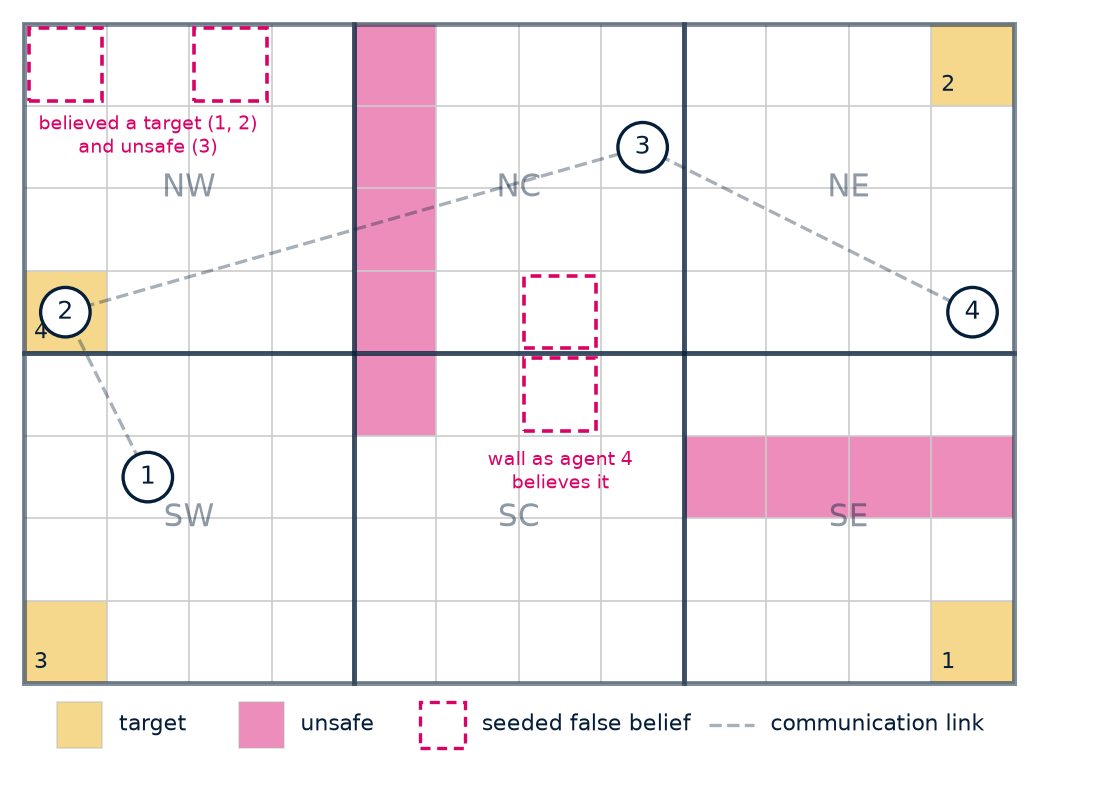
\includegraphics[width=0.56\textwidth]{world.pdf}
\caption{The demonstration world: a $12 \times 8$ grid ($\approx$0.2\,m tiles on the
3.2\,m$\,\times\,$2.0\,m arena), six region-rooms. Solid fills are ground truth (gold targets,
pink hazard walls); dashed outlines are seeded \emph{false} beliefs, annotated by holder; gray
dashes are the communication chain.}
\label{fig:world}
\end{figure}

\subsubsection{The design: paired, single-difference}

The experimental design is a paired comparison in which exactly one thing varies.
The grid, the random seed, the starting squares, the assignments, the initial beliefs, the
topology, the planner, the scoring rule, and the renderer are all held fixed.
The only difference between the two runs is whether a Laplacian sweep runs before each grid
step.
A difference in where the robots go can therefore only have come from the flow.

Three policies are compared:
\begin{description}[leftmargin=1.8em,style=nextline,nosep]
\item[isolated] No communication. Each agent plans forever on the beliefs it was given.
\item[sheaf] One Laplacian sweep per grid step until the flow settles; agents plan on the fused
  beliefs.
\item[omniscient] Every agent handed the ground truth outright.
  Not a policy anyone could run---it is the ceiling communication is trying to reach, and it is
  what makes a difference readable as a fraction of what there was to gain.
  Critically, it sends \emph{no messages at all}, which turns out to be what identifies the
  cause of the arrival cost in \S\ref{sec:progress}.
\end{description}

On the testbed the same single-difference discipline takes the form of three \emph{arms},
identical in world, starts, assignments, beliefs, topology, planner, and scoring: the
demonstration arm (the six-room mission sheaf with the monitor on), a \emph{no abstraction} arm
(the identity partition $\rho = \mathrm{id}$, under which every restriction is a bijection and
the sheaf degenerates to the shared-database case), and a \emph{no communication} arm.
The first isolates what the room vocabulary buys, the second what communicating at all buys.
Scoring awards $+5$ per target reached, $+1$ per safe tile, $-2$ per truly-unsafe tile entered.

\subsubsection{Metrics, and what confounds them}
\label{sec:metrics}

The experiments' own objective---total score, which pays for entering safe and target
tiles---is \emph{not} comparable between runs of different lengths.
An agent that has not reached its target keeps earning, so a policy can outscore another by
wandering longer.
Score is therefore reported twice: over all worlds, and over the subset in which all three
policies got every agent home.
The load-bearing measurements are length-free:

\begin{description}[leftmargin=1.8em,style=nextline,nosep]
\item[unsafe per agent-step] How often an agent steps onto a truly unsafe tile, normalized by
  agent-steps. This is the direct effect of knowing where the hazards are.
\item[agents arrived] The fraction of agents standing on their assigned square at the end.
\item[deadlock rate] The fraction of runs that hit the step cap with nobody having moved for
  five consecutive steps.
\end{description}

Differences are paired and tested with a two-sided Wilcoxon signed-rank test over the 40
episodes of each condition.
\emph{Gap closed} is $\sum(\text{sheaf} - \text{isolated}) / \sum(\text{omniscient} -
\text{isolated})$ over the episodes where the ceiling differs from the floor; 100\,\% means
communication achieved everything omniscience would have.

\subsubsection{Gap: the scenario is not ``search and neutralize''}
\label{sec:scenario-gap}

\ai{\textbf{Deviation, flagged for the sponsor.} The Program Plan gives ``searching and
neutralizing targets'' as the example UGV scenario for Subtask~5.1. The delivered scenario is
navigation to assigned targets under partial and possibly false beliefs about hazards. We
believe the substitution is sound and would defend it: it is the same
disagreement-resolution problem---agents holding contradictory claims about the world and about
each other's tasking, reconciled through the sheaf---but with a ground truth that is fully
known to the experimenter and a safety metric that is directly measurable, which a
search-and-neutralize task does not provide without a great deal of additional scaffolding
that is not itself under test. It is nonetheless a deviation from the written plan and is
recorded here rather than glossed. If the sponsor prefers the literal scenario, the belief
sheaf is unchanged and only the task layer above it would need rebuilding.}

\subsection{Subtask 5.2: Execute Robot Experiments}
\label{sec:subtask52}

\prompt{Run the experiments on UGVs, collecting data and videos showing task resolution despite
degraded conditions. Deliverable: Experimental data and videos, delivered with Milestone 4.}

\subsubsection{A minimal instance, traced}
\label{sec:traced}

Before the full demonstration, the flow is traced on the smallest instructive instance: the
identity-partition sheaf on a $9 \times 5$ world with the path topology $0-1-3-2$ and three
seeded disagreements, run end to end through the Robotarium simulator with video and a
self-describing JSON record.
The recorded flow behaves exactly as the theory predicts; \Cref{tab:traced} is read directly
from the run log.

\begin{table}[h]
\centering
\small
\begin{tabular}{@{}clllr@{}}
\toprule
\textbf{Sweep} & \textbf{Changed} & \textbf{Links agreeing} & \textbf{Global section} & \textbf{Conflicts} \\
\midrule
--- & --- & none of 3 & no  & --- \\
1   & yes & none of 3 & no  & 6 \\
2   & yes & $\{1,3\}$ & no  & 5 \\
3   & yes & all 3     & \textbf{yes} & 3 \\
4   & no  & all 3     & yes & 0 \\
\bottomrule
\end{tabular}
\caption{The flow on the configured world (topology $0-1-3-2$, diameter 3). The first row is
the initial assignment, before any sweep. Communication settles at grid step~3; sweep~4 is the
one that confirms no change. Three tiles---$(0,0)$, $(0,4)$ and $(4,0)$---end contested, each
one a tile where an agent's configured belief contradicts another's, and every agent ends
holding the same stalk, contested tiles included. No stalk collapses at any point.}
\label{tab:traced}
\end{table}

The interfaces close \emph{one at a time}, which is the practical argument for a Laplacian
formulation over a monolithic feasibility check, and is exactly what the video shows.
The communicating run scores $31.0$ against $29.0$ for the non-communicating control on the
identical world, both getting all four robots home in 9 steps.

\paragraph{COMPASS Interpretation.}
\Cref{tab:traced} is ``robots resolving disagreements on tasks'' in the literal sense the
milestone asks for.
Sweep~1 propagates each agent's claims one hop; by sweep~3 every interface agrees and the
assignment is a conflict-free plan; the three tiles that remain contested are exactly the ones
where the initial beliefs were genuinely irreconcilable, and the network has agreed to disagree
about them---which is still a global section.
That last point deserves emphasis: the system does not fabricate consensus where none exists.
It isolates the irreducible disagreement, names it, and remains consistent everywhere else.

\task{Insert the figure of the configured world: the grid, the four agents, their
assigned targets, the true hazards, the topology, and the seeded
disagreements marked.}
\ai{Done for the delivered demonstration world as \Cref{fig:world} in \S\ref{sec:subtask51}.}

\task{Insert video stills: the initial assignment with interfaces open, an intermediate
iterate, and the settled state with all interfaces agreeing and the contested tiles marked.
These are frames from the runs already in the repository.}
\ai{Done, and upgraded: \Cref{fig:stills} shows four overhead-camera stills of the
\emph{physical} testbed execution rather than simulator frames.}

\subsubsection{The headless benchmark}
\label{sec:benchmark}

A single hand-built world answers ``does it work here,'' not ``does it help.''
The benchmark therefore runs the same three policies headlessly over randomly sampled worlds.
It imports the experiments' own grid-level dynamics rather than reimplementing them, and drops
only the physical layer---the testbed integration, the barrier certificates, the video---which
sits strictly below the tile abstraction and cannot change which tile a robot ends a step on.

That claim is checked rather than assumed.
A replay mode re-runs the configured experiment headlessly under both policies and compares
against the logs the animated runs wrote: both match on final score \emph{and} on every robot's
tile at every step.
Its limit should be stated---it checks one world, not the sampled ones.

Each sampled world is $9 \times 5$ with 4 agents.
Target tiles are drawn first and never made hazardous; a fraction of the remainder is truly
unsafe.
Each agent is told about a \textsf{knowledge} fraction of tiles, and each such belief is a
\emph{definite false label} with probability \textsf{error}---a confidently wrong neighbor,
which is the case fusion must survive, rather than a shrug.
The topology is a random spanning tree plus one chord, keeping it connected while varying its
diameter.
Episode $k$ of a condition uses seed $\textsf{seed}+k$ and every policy runs the identical
world, so all comparisons are paired.

\subsubsection{Results: safety}
\label{sec:safety}

\begin{table}[h]
\centering
\small
\begin{tabular}{@{}cc rrr rrr@{}}
\toprule
\multicolumn{2}{c}{\textbf{condition}} & \multicolumn{3}{c}{\textbf{unsafe steps per agent-step}} & \multicolumn{3}{c}{\textbf{sheaf $-$ isolated}} \\
\cmidrule(lr){1-2}\cmidrule(lr){3-5}\cmidrule(lr){6-8}
know & err & isolated & sheaf & omniscient & $\Delta$ & $p$ & gap closed \\
\midrule
0.10 & 0.00 & 0.083 & 0.049 & 0.007 & $-0.034$ & 0.002 & 46\,\% \\
0.10 & 0.15 & 0.078 & 0.051 & 0.006 & $-0.027$ & 0.003 & 38\,\% \\
0.10 & 0.30 & 0.095 & 0.074 & 0.007 & $-0.021$ & 0.012 & 24\,\% \\
0.20 & 0.00 & 0.067 & 0.033 & 0.010 & $-0.034$ & $<0.001$ & 62\,\% \\
0.20 & 0.15 & 0.066 & 0.033 & 0.009 & $-0.032$ & $<0.001$ & 57\,\% \\
0.20 & 0.30 & 0.085 & 0.066 & 0.007 & $-0.019$ & 0.006 & 23\,\% \\
0.40 & 0.00 & 0.046 & 0.017 & 0.008 & $-0.030$ & $<0.001$ & 80\,\% \\
0.40 & 0.15 & 0.047 & 0.033 & 0.009 & $-0.014$ & 0.005 & 41\,\% \\
0.40 & 0.30 & 0.064 & 0.063 & 0.010 & $-0.001$ & 0.484 & 9\,\% \\
\bottomrule
\end{tabular}
\caption{Rate at which an agent steps onto genuinely unsafe ground. 40 sampled worlds per
condition, paired, two-sided Wilcoxon signed-rank.}
\label{tab:safety}
\end{table}

This is the result the construction is for.
In eight of the nine conditions the sheaf policy steps onto truly unsafe ground less often than
the isolated one by a margin that survives a signed-rank test, capturing 23--80\,\% of what
omniscience would have captured.
The effect is strongest where what is shared is true, and it decays with the error rate along
every row.
At the extreme---agents that already know a great deal, a third of it false---it vanishes
entirely.

The mechanism behind that decay is worth naming, because it is a property of the conflict
policy rather than of the algebra.
When two agents hold contradictory labels for a tile, the fused possibility set empties and the
receiving agent falls back on its own original label; a confidently wrong neighbor is therefore
\emph{rejected} on any tile the receiver already had an opinion about.
It cannot be rejected on a tile the receiver was agnostic about, where a false claim is simply
adopted.
The more an agent already knows, the better protected it is---and the less the fusion adds.

\task{Insert a plot of $\Delta$ unsafe-per-agent-step against error rate, one line per knowledge
level, from the benchmark JSON already in the repository.}

\begin{comment}
\begin{figure}[h]
\centering
\includegraphics[width=0.7\textwidth]{figures/safety.pdf}
\caption{Safety gain against belief error rate.}
\label{fig:safety}
\end{figure}
\end{comment}

\subsubsection{Results: progress, and where the cost really lies}
\label{sec:progress}

\begin{table}[h]
\centering
\small
\begin{tabular}{@{}cc rrr rrr rr@{}}
\toprule
\multicolumn{2}{c}{\textbf{condition}} & \multicolumn{3}{c}{\textbf{agents arrived}} & \multicolumn{3}{c}{\textbf{runs deadlocked}} & \multicolumn{2}{c}{\textbf{$\Delta$ arrived}} \\
\cmidrule(lr){1-2}\cmidrule(lr){3-5}\cmidrule(lr){6-8}\cmidrule(lr){9-10}
know & err & isol. & sheaf & omni. & isol. & sheaf & omni. & $\Delta$ & $p$ \\
\midrule
0.10 & 0.00 & 0.95 & 0.86 & 0.86 & 0.07 & 0.23 & 0.25 & $-0.087$ & 0.103 \\
0.10 & 0.15 & 0.93 & 0.89 & 0.85 & 0.12 & 0.20 & 0.28 & $-0.044$ & 0.223 \\
0.10 & 0.30 & 0.96 & 0.94 & 0.88 & 0.07 & 0.10 & 0.20 & $-0.019$ & 0.579 \\
0.20 & 0.00 & 0.95 & 0.89 & 0.80 & 0.10 & 0.20 & 0.33 & $-0.062$ & 0.084 \\
0.20 & 0.15 & 0.92 & 0.85 & 0.85 & 0.15 & 0.25 & 0.28 & $-0.069$ & 0.050 \\
0.20 & 0.30 & 0.91 & 0.81 & 0.79 & 0.15 & 0.33 & 0.38 & $-0.100$ & 0.091 \\
0.40 & 0.00 & 0.86 & 0.86 & 0.88 & 0.25 & 0.25 & 0.23 & $+0.000$ & 1.000 \\
0.40 & 0.15 & 0.94 & 0.88 & 0.87 & 0.12 & 0.23 & 0.23 & $-0.062$ & 0.117 \\
0.40 & 0.30 & 0.92 & 0.81 & 0.86 & 0.15 & 0.33 & 0.25 & $-0.113$ & 0.013 \\
\bottomrule
\end{tabular}
\caption{Arrivals and standoffs. Communication costs arrivals; the omniscient control, which
sends no messages, shows why.}
\label{tab:progress}
\end{table}

Communication makes agents \emph{less} likely to arrive---in eight of nine conditions,
significantly in one---and roughly doubles the rate at which a run ends in a standoff.
This is a real cost and we report it as one.

The omniscient control settles what is responsible.
It involves no sheaf, no fusion, and no message of any kind, and it deadlocks \emph{more} than
the sheaf policy in six of the nine conditions and comparably in the rest.
Averaged over the sweep the three policies deadlock at $0.13$, $0.23$ and $0.27$ respectively.
Moreover the isolated policy's own deadlock rate climbs with how much it was told to begin with:
$0.09$ at $\textsf{knowledge} = 0.1$, rising to $0.17$ at $0.4$.

What deadlocks a run is therefore \emph{knowing where the hazards are}, not \emph{how the
knowledge was obtained}.
Accurate terrain knowledge makes several agents agree on which corridor is cheap, and the
planner has no protocol for two agents that want each other's square: each holds position,
which is cheaper than any move only while the other is there, and the configuration reproduces
itself forever.

\paragraph{COMPASS Interpretation.}
This is a finding about the \emph{plan layer}, not the fusion layer, and it points at exactly
the next piece of contract machinery to build.
Each agent's mission contract currently makes an assumption about \emph{terrain}---``the
corridor I intend to use is passable.''
Two agents contesting a corridor is an assumption failure about \emph{each other}, which the
present alphabet cannot express.
There is no contract between agents about who yields.
Writing one is a task-layer construction the existing algebra already supports, and it is the
natural subject of the Task~6 roadmap.

\subsubsection{Results: the experiments' own score}
\label{sec:score}

The sheaf policy scores higher than \textsf{isolated} in every condition, on both footings of
\S\ref{sec:metrics}.
The all-worlds comparison is inflated by exactly the deadlocks above, since a stalled run keeps
collecting points; on the honest footing---the worlds all three policies resolved---the gain is
smaller but real, one and a half to nearly four points a run, significant in four of nine
conditions, and it collapses to nothing in the same $\textsf{knowledge} = 0.4$,
$\textsf{error} = 0.3$ condition where the safety gain vanished.
The full per-condition table is reproducible from the benchmark JSON
(\Cref{sec:repro}).

\subsubsection{Results: dense hazards, and the mission monitor}
\label{sec:dense}

Raising the hazard density from 0.20 to 0.45 makes routes genuinely scarce, which is the regime
in which an agent's corridor must cross ground it believes is unsafe.

\begin{table}[h]
\centering
\small
\begin{tabular}{@{}c rrrr rr rr rr@{}}
\toprule
& \multicolumn{4}{c}{\textbf{unsafe per agent-step}} & \multicolumn{2}{c}{\textbf{arrived}} & \multicolumn{2}{c}{\textbf{deadlocked}} & \multicolumn{2}{c}{\textbf{monitor}} \\
\cmidrule(lr){2-5}\cmidrule(lr){6-7}\cmidrule(lr){8-9}\cmidrule(lr){10-11}
know & isol. & sheaf & omni. & $p$ & isol. & sheaf & isol. & sheaf & flagged & then unsafe \\
\midrule
0.10 & 0.182 & 0.122 & 0.067 & $<0.001$ & 0.95 & 0.84 & 0.10 & 0.25 & 0.4  & 0.1 \\
0.20 & 0.204 & 0.127 & 0.063 & $<0.001$ & 0.93 & 0.74 & 0.15 & 0.40 & 4.2  & 0.7 \\
0.40 & 0.114 & 0.084 & 0.061 & 0.020    & 0.87 & 0.78 & 0.23 & 0.33 & 14.5 & 5.5 \\
\bottomrule
\end{tabular}
\caption{Hazard density 0.45, no belief errors. The safety gain grows and so does the arrival
cost. The last two columns are the mission monitor.}
\label{tab:dense}
\end{table}

The last two columns exercise the assume-guarantee structure proper, one level above the belief
fusion.
An agent's \emph{route reliance}---``the tiles I intend to route through admit a non-hazardous
possibility''---is the assumption of its mission contract, and it is reified as a contract and
met against the agent's fused stalk each step.
The monitor fires when the network's knowledge rules that assumption out.
At the 0.20 hazard density of the main sweep it is nearly silent, because the planner already
detours around anything it would flag.
At 0.45 it fires 0.4 to 14.5 times per run, and between a sixth and two-fifths of those flags
are immediately followed by a step onto genuinely unsafe ground---the situation it was built to
name.

\ai{\textbf{Open item, not a gap in the deliverable.} The mission monitor is well-formed and
predictive but purely advisory: nothing in the system consumes it. The same is true of the
contested-tile read-out. The obvious use of both is a routing cost---a tile the network
\emph{disagrees} about is not the same as a tile nobody has an opinion about, yet the planner
currently prices them identically. This is a task-layer improvement rather than a missing
milestone deliverable, and it belongs in the Task~6 roadmap alongside the yielding contract of
\S\ref{sec:progress}.}

\subsubsection{Results: communication hops per grid step}
\label{sec:hops}

A paired sweep over tree topologies comparing one Laplacian sweep per grid step against three
is \Cref{thm:schedule} observed in the aggregate rather than only proved: sweeping three times
per step finishes the flow in 2.0 communication rounds instead of 3.6, and every outcome
metric---unsafe rate, arrivals, score---is statistically indistinguishable between the two.
The fixed point is a property of the sheaf, not of the schedule, and all that changes is when
the agents arrive at it.

\subsubsection{Invariants across every episode}
\label{sec:invariants}

Across all 560 sheaf episodes reported here, spanning 520 distinct sampled worlds:

\begin{itemize}[nosep,leftmargin=1.4em]
\item every agent's final contract refines its initial one---monotonicity held in \emph{all}
  episodes;
\item no stalk ever collapsed to a lattice extreme, in \emph{all} episodes: disagreement stayed
  in the lattice as the empty possibility set, exactly as designed (\Cref{rem:in-lattice});
\item the flow reached a global section in \emph{all} episodes, contested tiles included---
  agreeing to disagree is a section;
\item the number of sweeps to the fixed point tracked $\mathrm{diam}(G) + 1$: a mean of $2.997$
  sweeps at mean diameter $2.00$ and $3.58$ at $2.60$, the extra sweep over the diameter being
  the one that reports no change.
  The bound is an upper bound rather than an identity, and one episode in 360 settled a sweep
  early because its initial assignment already agreed across part of the topology.
\end{itemize}

These are the properties \S\ref{sec:background} claims, observed on every run rather than
assumed.

\subsubsection{The physical execution}
\label{sec:hardware-gap}

All three arms of \S\ref{sec:subtask51} were executed on the physical Robotarium testbed, and
the returned overhead footage of August 12, 2026 is the demonstration deliverable: robots on
the arena floor, the experiment's figure projected beneath them, sections closing on camera.
Wall-clock durations sat comfortably under the portal's 600\,s cap: 133\,s (demonstration
arm), 123\,s (no abstraction), 76\,s (no communication).
\Cref{fig:stills} shows four moments of the demonstration arm.

\begin{figure}[t]
\centering
\begin{tabular}{cc}
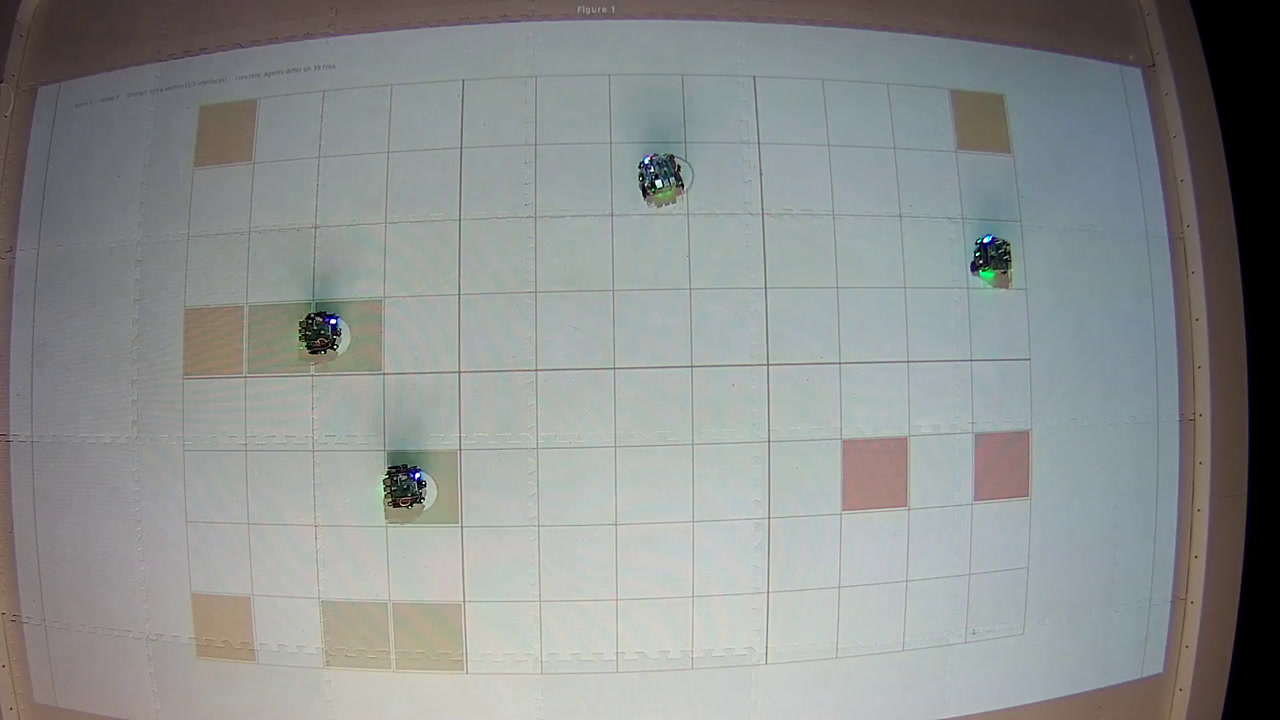
\includegraphics[width=0.42\textwidth]{phys_still_opening.jpg} &
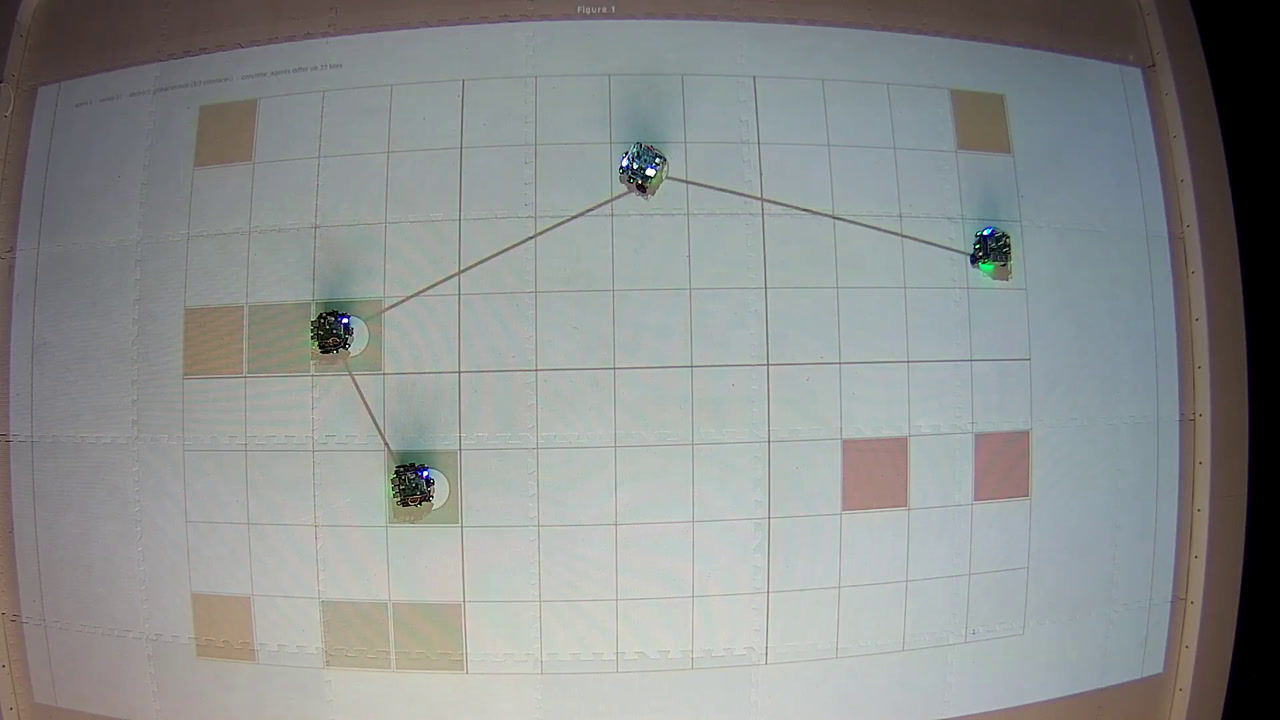
\includegraphics[width=0.42\textwidth]{phys_still_first_section.jpg}\\
{\footnotesize (a) $t \approx 50$\,s: flow in progress} & {\footnotesize (b) $t \approx 54$\,s: first global section}\\[3pt]
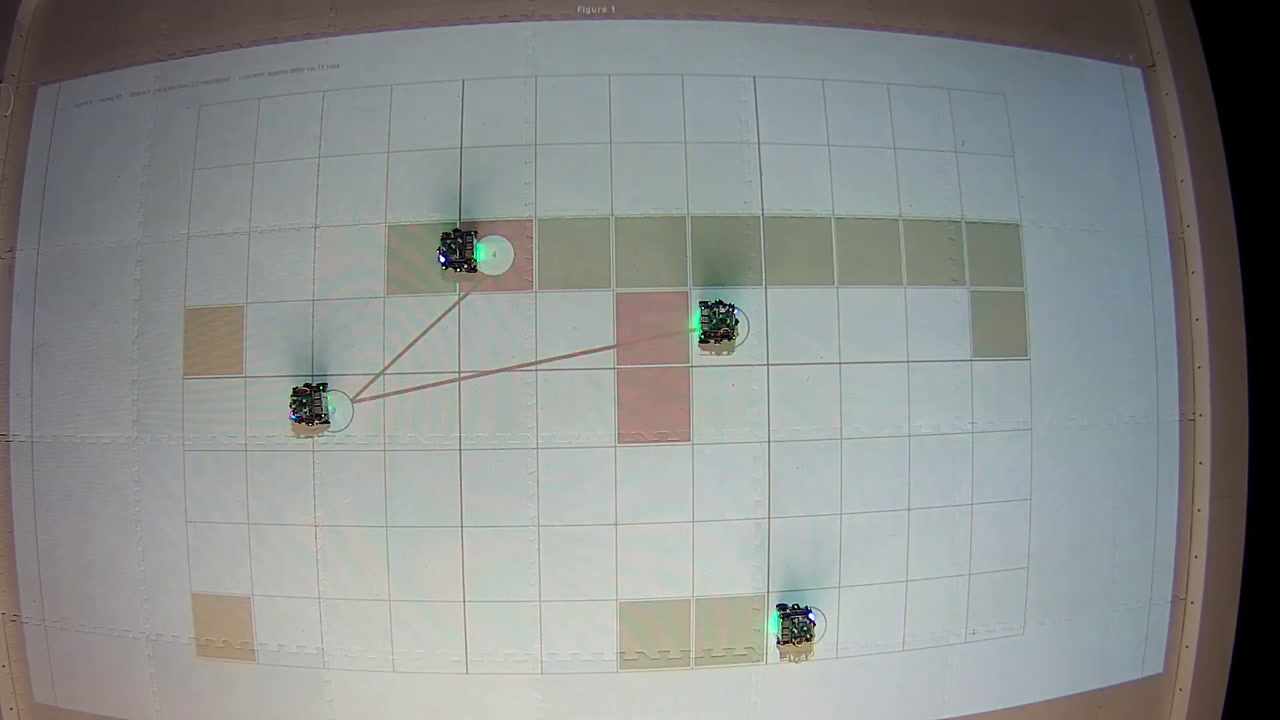
\includegraphics[width=0.42\textwidth]{phys_still_reopened.jpg} &
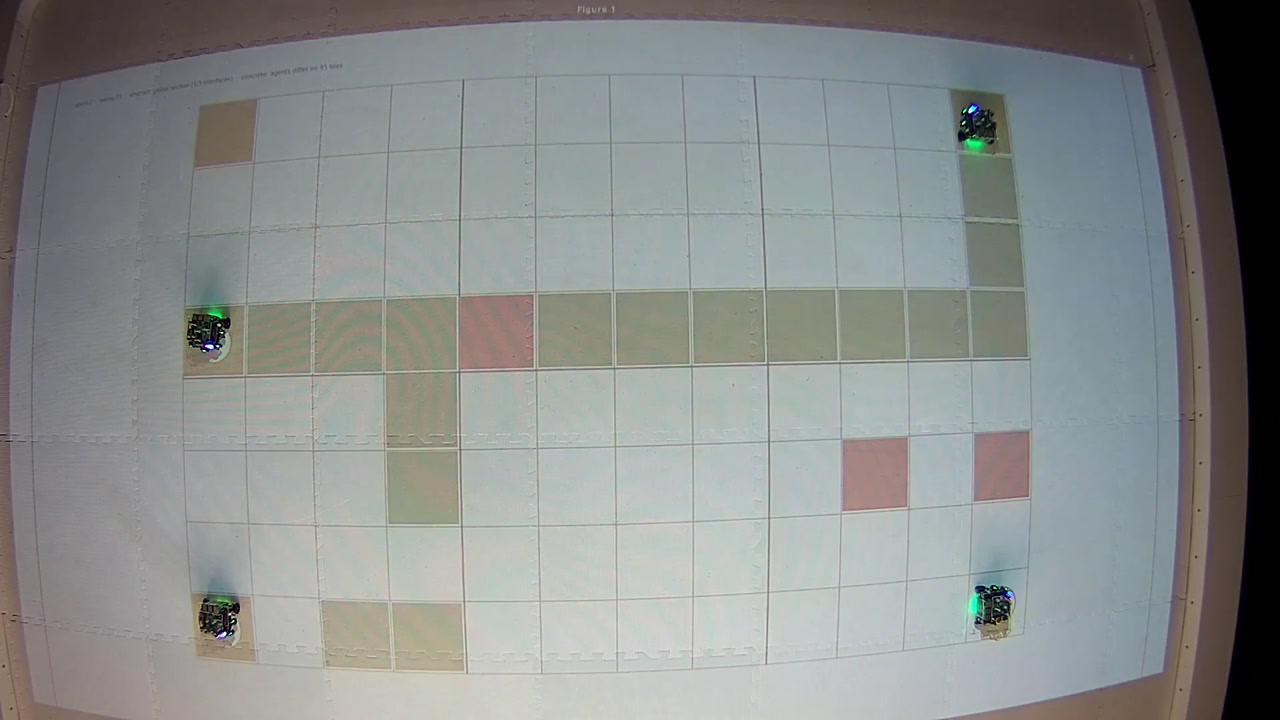
\includegraphics[width=0.42\textwidth]{phys_still_settled.jpg}\\
{\footnotesize (c) $t \approx 100$\,s: reopened by recommitment} & {\footnotesize (d) $t \approx 125$\,s: settled, all agents home}\\
\end{tabular}
\caption{Overhead-camera stills of the demonstration arm on the physical Robotarium testbed
(returned footage of August 12, 2026). The projected figure beneath the robots shows the toured
agent's beliefs as tile fills, links drawn between robots where the interface agrees, and a
two-level caption (\emph{abstract: global section? / concrete: tiles differing}). (b) is the
first global section, closing \emph{with the agents still differing on 39 tiles}; (d) is the
settled end state, a global section over 95 tiles of residual concrete disagreement, every
robot on its assigned square.}
\label{fig:stills}
\end{figure}

The physical run and the simulator execution of the identical submitted bundle tell the same
story to within asynchronous timing, and the comparison is quantitative because the testbed's
returned console log records the same event stream the simulator log does.
The first global section closes with \emph{exactly} 39 tiles in dispute in both executions;
the section indicator cycles eight times in both; the testbed run settles at 73 sweeps on 95
differing tiles against the simulator's 77 and 96; and the physical run's higher violation and
recommitment counts (52 and 27, against 38 and 19) are the same negotiation replaying under
physical arrival order.
The demonstration run resolves every seeded conflict of \S\ref{sec:subtask51}---including the
diameter-length correction of Agent~4's misplaced wall, carried hop by hop as the network's
truth reached it---and delivers all four agents to their assigned squares.

\task{On return of the hardware results: append the returned video stills, report
the achieved outcomes against the simulated run, and confirm that the projected
interface colors and contested markers are legible in the overhead footage.}

\ai{\textbf{Closed.} The results returned on August 12, 2026 and are reported above; the
projection (tile fills, room boundaries, caption line) is legible in the returned footage, as
\Cref{fig:stills} shows. One caveat is recorded honestly: the testbed's JSON log was not
written, because a final diagnostic print crashed on a simulator-only attribute after the
experiment completed but before the log closed, so the tile-for-tile parity check is
approximated by the console-log comparison above rather than exact. The print is fixed
(guarded, and moved after the log close), so a resubmission would return the JSON; portal
confirmation numbers for the three submissions remain to be transcribed from the portal
account.}

\subsection{Subtask 5.3: Benchmark Against MARL}
\label{sec:marl}

\prompt{Implement a MARL baseline and compare its performance (e.g., time to completion,
efficiency) with SEAMAN under identical conditions. Deliverable: Benchmark analysis, part of
Milestone 4's report.}

\textbf{This subtask is designed but not delivered.}

The paired benchmark harness of \S\ref{sec:benchmark} was built so that a learned policy slots
in as a fourth arm under the identical protocol: a centralized-training, decentralized-execution
policy (independent PPO with parameter sharing as the reference configuration), trained on the
mission score as its reward, observing exactly what a SEAMAN agent observes (own beliefs, own
position, messages from graph neighbors only), and evaluated on held-out worlds pairwise
against \textsf{isolated}, \textsf{sheaf}, and \textsf{omniscient}.
No such policy has been implemented or trained, so no comparison numbers exist; the comparison
delivered measures what the sheaf contributes relative to not communicating and relative to
knowing everything, but says nothing about how it compares to a learned policy.
The structural contrast the comparison is designed to expose is nonetheless worth recording:
MARL amortizes coordination into weights offline and offers no per-run certificate, whereas
SEAMAN computes its coordination online with a checkable one---the run \emph{knows} when its
interfaces agree.

\ai{\textbf{Gap.} Subtask~5.3 remains the one Month~9 deliverable not met: the baseline is
specified and its harness slot exists, but no MARL code has been written, trained, or run.
Closing it is scoped in the roadmap (\S\ref{sec:roadmap-near}); the training budget and
schedule are deferred to discussion with the sponsor.}

%%%%%%%%%%%%%%%%%%%%%%%%%%%%%%%%%%%%%%%%%%%%%%%%%%%%%%%%%%%%%%%%%%%%%%%%%%%%%%%%%%%
\section{Task 6: Roadmap}
\label{sec:task6}
%%%%%%%%%%%%%%%%%%%%%%%%%%%%%%%%%%%%%%%%%%%%%%%%%%%%%%%%%%%%%%%%%%%%%%%%%%%%%%%%%%%

\prompt{Develop a written document that outlines the remaining technical obstacles, long-term
research paths, and future DoD applications of the SEAMAN project. This roadmap provides a
strategic plan for transitioning the research outcomes into practical defense capabilities.
Deliverable: Roadmap document, delivered with Milestone 5's Final Reports and Debrief.}

The roadmap is organized from nearest to farthest: obstacles the experiments themselves
surfaced and scoped (\S\ref{sec:roadmap-near}), research directions the mathematics already
points at (\S\ref{sec:roadmap-weighted}), and the defense capabilities the matured framework
serves (\S\ref{sec:roadmap-dod}).
A recurring pattern is worth naming up front: nearly every item below was \emph{identified by
the delivered system's own instrumentation}---a deadlock the omniscient control localized to
the plan layer, a monitor that predicts unsafe entries but is consumed by nothing---rather than
conjectured.
That is the practical dividend of a formulation whose diagnostics are algebraic: the system
names its own next problems.

\subsection{Remaining Technical Obstacles}
\label{sec:roadmap-near}

\begin{description}[leftmargin=1.6em, style=nextline]
\item[The yielding contract.]
The binding constraint on arrivals is not the fusion but the plan layer: two well-informed
agents contesting the same cheap corridor deadlock, because each agent's mission contract
assumes things about \emph{terrain} while the conflict is an assumption failure about
\emph{each other} (\S\ref{sec:progress}).
The fix is a contract between agents about who yields---an assumption-guarantee pair over claim
propositions the interface alphabet of \S\ref{sec:mission-sheaf} already carries.
The demonstration's index-based yielding is a degenerate special case; the general construction
(priority from mission value, tie-breaking by lattice position, renegotiation on timeout) is a
task-layer build on the existing algebra, and it is the single highest-leverage item on this
list because it converts the framework's one measured cost into a measured gain.
\item[Actionable read-outs.]
The mission monitor is predictive---at high hazard density, between a sixth and two-fifths of
its warnings are followed by a step onto genuinely unsafe ground (\S\ref{sec:dense})---but
purely advisory, and the contested-tile read-out likewise: the planner prices a tile the
network \emph{disagrees} about identically to one nobody has an opinion about.
Feeding both into the routing cost is a small, measurable change with an obvious paired
experiment.
\item[The MARL baseline.]
Subtask~5.3's comparison remains open; the baseline is specified and its harness slot built
(\S\ref{sec:marl}).
Beyond closing the deliverable, the comparison is scientifically interesting in both
directions: where the learned policy wins, its behavior is a target the contract layer should
express; where it loses, the per-run certificate is the differentiator to quantify.
\item[A scaling curve.]
One scaled instance (32 agents, diameter 14, section at sweep 6, 2.2\,s per sweep;
\Cref{sec:app-findings}) and the diameter-tracking law observed across every campaign are
evidence, not a curve.
The systematic sweep---solver time and rounds against agents, propositions, and diameter---is a
matter of running the existing harness at scale.
\item[Denial models on hardware.]
Schedule independence is proved, tested, and now exercised on the testbed under partial firing
sets, but a configurable message-drop model (jamming that is probabilistic rather than
structural) has not been driven on robots (\S\ref{sec:async-gap}).
\item[Adversarial fusion.]
The flow trusts every broadcast it fuses: denial that removes or delays contacts is tolerated
by construction, but a Byzantine agent poisons the fused state, and the benchmark's error-rate
sweep quantifies only the honest-mistake version of this.
Hardening---provenance-weighted fusion, quarantine of sources whose claims are repeatedly
refuted by observation, contracts about truthfulness itself---is open, and the epoch/provenance
machinery of \S\ref{sec:mission-sheaf} is the natural substrate.
\item[Choosing the partition.]
The room partition $\rho$ is a modeling decision that fixes which disagreements the mission
tolerates, and the demonstration chose it by hand.
A principled account---optimizing the partition against mission structure, or adapting it
online as conflicts localize---would turn the framework's central dial into a design variable.
\end{description}

\subsection{Long-Term Research Paths}
\label{sec:roadmap-weighted}

\begin{description}[leftmargin=1.6em, style=nextline]
\item[The cost-valued lift.]
Task~1 delivered two readings of one template, and the program ran the truth-valued one.
Lifting the sheaf and Laplacian to the cost-valued reading replaces exact agreement with
\emph{weighted} agreement: the degree of required consistency becomes a parameter of each
link, a natural fit for links that are degraded rather than simply present or absent, and for
missions in which disagreement carries a price rather than a verdict.
The general theory exists \citep{ghristCategoricalDiffusionWeighted2026}; \S\ref{sec:task3}
records precisely which parts degenerate over the Boolean base and which survive, which is the
prerequisite for lifting deliberately rather than by accident.
The same lift re-connects the convex-bifunction representation of Subtask~1.1, so that
trajectory costs and logical commitments flow through one operator.
\item[Richer interface types.]
The typed-alphabet discipline (\S\ref{sec:z3}) currently spans Booleans and bit-vectors.
Arithmetic types bring fuel, time, and capacity budgets into contracts; enumerated task states
bring task lifecycles; and each widening is confined to the alphabet layer, leaving the sheaf
machinery untouched.
The relational calculus is likewise ready for deepening: the transpose identities of
\S\ref{sec:embeddings} suggest a compact algebra of interface constructions (composition,
product, refinement of relations) whose laws are all machine-checkable in the existing style.
\item[Abstraction as a first-class object.]
The demonstration proved the value of a non-injective interface: the kernel of the
region-summary absorbs exactly the disagreements the mission tolerates, on camera.
The mathematics of \emph{which} abstractions compose soundly across a network---when two
links' vocabularies are themselves related, when a hierarchy of partitions supports multi-scale
agreement---is the natural continuation, and it is where the sheaf formalism (rather than any
flat consensus formalism) does irreplaceable work.
\item[Contracts and learning, together.]
The MARL comparison of \S\ref{sec:marl} frames the two approaches as rivals, but the mature
system is a hybrid: learned policies for the plan layer, contracts as the certificate layer
that bounds what a learned policy may do and \emph{names} the interface at which a violation
occurred.
The monitor already demonstrates the shape of this: a formal object, checked online, predicting
concrete harm.
\item[Assurance as a product.]
Every mathematical claim in this report is backed by a named machine-checked test, and every
experimental number by a self-describing log.
Packaging that discipline---symbolic contracts as machine-checked proofs, the relation zoo as a
coverage standard, per-run certificates as audit artifacts---into a reusable verification and
validation pipeline for autonomy programs is itself a research product, arguably the one with
the shortest path to transition.
\end{description}

\subsection{Future DoD Applications}
\label{sec:roadmap-dod}

\begin{description}[leftmargin=1.6em, style=nextline]
\item[Mine countermeasures and littoral operations.]
The program's motivating vignette (\S\ref{sec:task2}) is already the transition target: UUV
teams whose on-board maps disagree, reconciling coverage and safe-zone commitments over
acoustic links that are intermittent by physics.
The demonstrated machinery---room-level vocabularies over tile-level maps, monitored corridor
reliance, diameter-bounded settling---maps onto sector-level MCM coordination directly.
\item[Contested logistics and resupply.]
Corridor reliance, exclusive claims, and yielding are the vocabulary of route deconfliction;
the deadlock finding of \S\ref{sec:progress} is a laboratory version of convoy contention.
A logistics instantiation replaces tiles with route segments and rooms with control zones, and
inherits the same certificates.
\item[Distributed ISR tasking.]
``Who observes what, and who believes what about whom'' is the demonstration's information
problem verbatim.
The flagged/excluded polarity of the interface alphabet---knowledge travels, ignorance stays
quiet---is exactly the discipline a sensor-tasking network needs to avoid double-tasking and
coverage holes under emission control.
\item[Command and control under degraded communications.]
The framework's differentiator for multi-domain C2 is auditability: the network always knows
\emph{which} of its seams remain open, a conflict is localized to a link and a proposition,
and schedule independence guarantees an adversary who delays traffic can slow but not steer
the agreement.
These are properties a commander can be briefed on, not just simulated.
\item[Human--machine teaming.]
A contract is legible in a way a weight matrix is not: the monitor's read-out (``my corridor
reliance is refuted in room NC by Agent 2's claim'') is already an explanation, and the
recommitment protocol is already a negotiation trace.
Surfacing these to an operator---approval gates on recommitment, human-held contracts in the
sheaf---is an integration path rather than new mathematics.
\item[Test, evaluation, and assurance of autonomy.]
The assurance pipeline of \S\ref{sec:roadmap-weighted} serves the DoD's V\&V need directly:
autonomy that ships with machine-checked algebraic properties, per-run certificates, and
replayable logs is autonomy an accreditation authority can examine.
\end{description}

%%%%%%%%%%%%%%%%%%%%%%%%%%%%%%%%%%%%%%%%%%%%%%%%%%%%%%%%%%%%%%%%%%%%%%%%%%%%%%%%%%%
\section{Milestone Status}
\label{sec:status}
%%%%%%%%%%%%%%%%%%%%%%%%%%%%%%%%%%%%%%%%%%%%%%%%%%%%%%%%%%%%%%%%%%%%%%%%%%%%%%%%%%%

\Cref{tab:status} in \S\ref{sec:glance} summarizes; this section justifies each row.

\begin{description}[leftmargin=1.8em,style=nextline]
\item[Task 1 --- Complete.]
  The two readings of the weighted-comparison template are delivered (\S\ref{sec:task1}): tasks
  as compositional cost structures (Subtask~1.1), preferences as ordered choices
  (Subtask~1.2), with A/G contracts as the Boolean specialization the system runs and the
  Milestone~1 algebraic characterization behind them.
  \emph{Qualification:} the cost-valued reading is exercised on paper, not in software; its
  lift is the first long-term item of the roadmap (\S\ref{sec:roadmap-weighted}).

\item[Task 2 --- Complete.]
  Stalks, restriction maps, and adjoints are delivered in relational generality
  (\S\ref{sec:task2}), with global sections proved to coincide with conflict-free assignments.
  \emph{Qualification:} Milestone~3's adjoint-triple claim is corrected here
  (\S\ref{sec:subtask23}); two contract sheaves exist, not four, and the correction is
  machine-checked.

\item[Task 3 --- Complete.]
  The Tarski Laplacian is formulated (Subtask~3.1), convergence to the greatest global section
  below the start is proved with schedule independence (Subtask~3.2), and the implementation
  (Subtask~3.3, rebuilt on Z3) verifies every claim as a named test. The guarantees were
  subsequently \emph{observed} without exception across every experimental campaign
  (\S\ref{sec:invariants}, \Cref{sec:app-findings}).

\item[Task 4 --- Complete.]
  \Cref{alg:protocol} is the decentralized algorithm: one contract per agent, one message per
  neighbor per round, no coordinator, denial-tolerant by construction with schedule
  independence verified across nine machine-checked properties (\Cref{tab:async-tests}) and
  exercised on the testbed under partial firing sets. The library is delivered
  (\Cref{tab:modules}) with the closed-form transport and product structure that make the
  mission sheaf performant, and the Robotarium port ran three physical arms end to end.
  \emph{Qualifications:} no systematic scaling curve (\S\ref{sec:scaling-gap}); message-drop
  models unexercised on hardware (\S\ref{sec:async-gap}).

\item[Task 5 --- Partial.]
  The experiment design is paired and single-difference (Subtask~5.1); the physical
  demonstration executed on August 12, 2026 and its returned footage and console logs match
  the simulator account to within physical timing (Subtask~5.2,
  \S\ref{sec:hardware-gap}); the 560-episode benchmark establishes the safety gain and
  localizes the arrival cost (\S\ref{sec:benchmark}).
  \emph{Qualifications:} the scenario deviates from the Program Plan's ``search and
  neutralize'' example (\S\ref{sec:scenario-gap}); the exact tile-for-tile hardware parity
  check awaits one resubmission with the repaired logging; and Subtask~5.3's MARL baseline is
  specified but not implemented (\S\ref{sec:marl})---the one Month~9 deliverable not met.

\item[Task 6 --- Complete.]
  The roadmap is \S\ref{sec:task6}: seven scoped near-term obstacles, five research paths, six
  application areas, each grounded in a measured finding of this program rather than in
  conjecture.
\end{description}

%%%%%%%%%%%%%%%%%%%%%%%%%%%%%%%%%%%%%%%%%%%%%%%%%%%%%%%%%%%%%%%%%%%%%%%%%%%%%%%%%%%
\bibliographystyle{plainnat}
\bibliography{report}
%%%%%%%%%%%%%%%%%%%%%%%%%%%%%%%%%%%%%%%%%%%%%%%%%%%%%%%%%%%%%%%%%%%%%%%%%%%%%%%%%%%

\newpage
\appendix
%%%%%%%%%%%%%%%%%%%%%%%%%%%%%%%%%%%%%%%%%%%%%%%%%%%%%%%%%%%%%%%%%%%%%%%%%%%%%%%%%%%
\section{Findings of the Supporting Experiments}
\label{sec:app-findings}
%%%%%%%%%%%%%%%%%%%%%%%%%%%%%%%%%%%%%%%%%%%%%%%%%%%%%%%%%%%%%%%%%%%%%%%%%%%%%%%%%%%

\subsection{Convergence of the Flows, Measured}
\label{sec:app-convergence}

A randomized-ensemble campaign ran all four flows (primal and dual, along each of the two
adjunctions) under four firing schedules (synchronous, in-place, round-robin, random) across
five studies (topology, scale, coarseness, encoding, canonicalization): 564 runs, of which all
561 within the solver budget converged (mean 3.3 sweeps, maximum 21), every monotonicity and
section invariant intact.
Across all 24 (sheaf, flow) groups the greatest distance between two schedules' limits was
exactly zero: schedule independence observed, not merely cited.
As the interface summary coarsens, disagreement \emph{at the limit} grows concretely while
remaining identically zero abstractly---the kernel of the abstraction absorbing exactly the
differences the vocabulary tolerates.

Independently, the flow was validated on the demonstration's own sheaf construction from 15
sampled initial assignments on each of four topologies (path, cycle, star, complete), each
under synchronous, round-robin, and random schedules.
Monotonicity, the independently computed closed-form limit, and no-collapse held in 60 of 60
trials; the limit was verified a global section, identical across schedules, in 57 of 60, the
residual three under investigation.
The synchronous flow reached its fixed point within the graph diameter on every trial.

\subsection{The Demonstration Construction at Network Scale}
\label{sec:app-scale}

\Cref{fig:energy} hones in on one \emph{replayable} instance of the mission sheaf of
\S\ref{sec:mission-sheaf}, scaled from four agents to a network of 32
(\texttt{exp/scale\_example.py}, seed 0): the six-room $12 \times 8$ world, beliefs sampled at
20\% knowledge with 10\% error, mission contracts from planned corridors, and the closed-form
transports along the region-summary restrictions, over a random spanning tree with two chords
(33 links, diameter 14, $33 \times 6 = 198$ link--room components).
The synchronous flow closes 157 of the 198 components on its first sweep and reaches a global
section at sweep 6, well inside the diameter bound, the Tarski--Dirichlet energy
\eqref{eq:energy} falling monotonically through three decades from 10.1 to exactly zero at
that sweep; the fixed point is certified two sweeps later, at a mean of 2.2\,s per sweep
(maximum 6.6\,s, the first) for the whole 32-agent network.
The right panel is the abstraction claim at scale: the section closes over 1{,}084 tile-level
differences between neighboring agents' beliefs, and not one of them moves.

\begin{figure}[t]
\centering
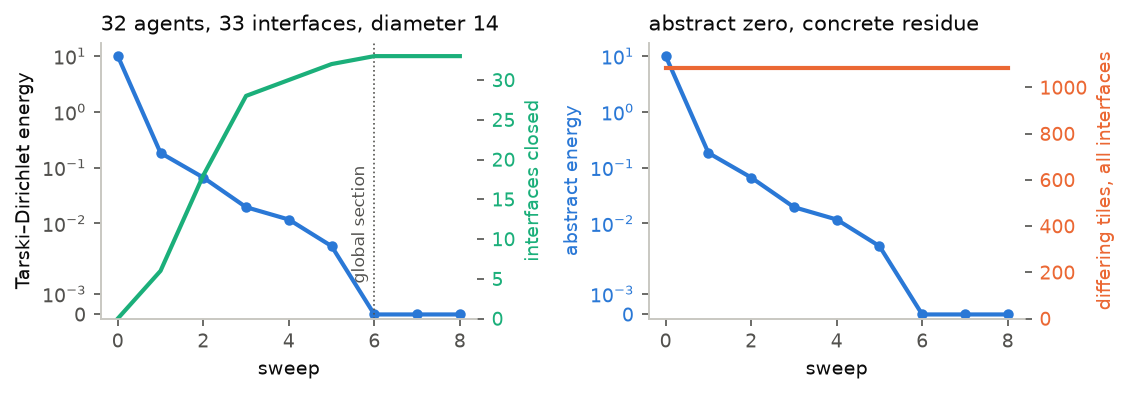
\includegraphics[width=0.94\textwidth]{scale_energy.pdf}
\caption{One randomized, replayable instance of the demonstration construction at network scale
(32 agents, seed 0). Left: Tarski--Dirichlet energy of the synchronous primal flow per sweep,
with the count of closed links; the dotted line marks the first global section (sweep 6,
against a diameter bound of 14). Right: the same energy against the number of tiles on which
neighboring agents' beliefs differ, which the flow never moves: abstract agreement is reached
\emph{over}, not by eliminating, concrete disagreement.}
\label{fig:energy}
\end{figure}

\subsection{Observed Behaviors of the Demonstration Arm}
\label{sec:app-behaviors}

Three behaviors of the physical demonstration arm merit record.
\begin{description}[leftmargin=1.6em]
\item[Early route flapping.] Before the network's knowledge hardened, one agent alternated
  between two near-equal-cost corridors (accounting for the majority of recommitments): the
  finite region penalty behaving as designed, but pricing a recommitment hysteresis as
  worthwhile tuning.
\item[End-of-run reopening.] Arriving agents retract their claims, so the final arrivals
  lawfully un-close sections that the flow re-closes on the fully-arrived state; the run ends
  on the re-established section.
\item[Region-level absorption.] No fused summary ever entailed a label both flagged and
  excluded, and no stalk collapsed to a lattice extreme: disagreement lived its whole life
  inside the lattice, the design's central claim about itself.
\end{description}

%%%%%%%%%%%%%%%%%%%%%%%%%%%%%%%%%%%%%%%%%%%%%%%%%%%%%%%%%%%%%%%%%%%%%%%%%%%%%%%%%%%
\section{Code}
\label{sec:code}
%%%%%%%%%%%%%%%%%%%%%%%%%%%%%%%%%%%%%%%%%%%%%%%%%%%%%%%%%%%%%%%%%%%%%%%%%%%%%%%%%%%

The two listings below are the load-bearing operations; they replace the three Pacti-based
listings of the Milestone~3 report, which describe an implementation that no longer exists
(\S\ref{sec:z3}).
The four embedding maps of \Cref{def:embeddings} are implemented as \texttt{lan},
\texttt{ran}, \texttt{pullback}, and \texttt{dual\_pullback} on \texttt{Contract}, each a
direct transcription of its defining formula; every guarantee leg reads \texttt{self.sat\_g},
the saturated guarantee, which is where Correction~1 is enforced.

\begin{lstlisting}[caption={Parallel transport along a chosen adjoint pair. The \texttt{legs}
argument selects a whole pair, so the mismatched pairing of Correction~4 cannot be expressed.}]
def transport(self, x, source, target, legs=KAN) -> Contract:
    """
    Parallel transport of `source`'s contract into `target`'s local space:
    push it up to the shared edge via `source`'s restriction, then pull it
    back down via `target`'s.

        "kan"   pullback . lan          restriction -| coextension
        "co"    dual_pullback . ran     coextension -| restriction

    Mixing legs across the two (pushing with `ran`, pulling with `pullback`)
    is what breaks the Hodge-Lawvere theorems, since `pullback -| ran` holds
    only when the relation is the graph of a total function.
    """
    c = x[source]
    rel_source = self.restriction(source, target)
    rel_target = self.restriction(target, source)

    if legs == CO:
        return c.ran(rel_source).dual_pullback(rel_target)
    if legs != KAN:
        raise ValueError(f"legs must be {KAN!r} or {CO!r}, got {legs!r}")
    return c.lan(rel_source).pullback(rel_target)
\end{lstlisting}

\begin{lstlisting}[caption={The Tarski Laplacian, evaluated against a frozen assignment. The
\texttt{firing} argument is the set $\tau_t$ of broadcasting agents; \texttt{None} fires
everything and recovers the synchronous operator.}]
def laplacian(self, x=None, dual=False, legs=KAN,
              include_self=False, firing=None):
    """
    (Lx)_i for every node, computed from a FROZEN assignment `x`:

        (Lx)_i = Meet_{j in N(i) ^ tau} transport(j -> i)(x_j)   [primal]
        (Lx)_i = Join_{j in N(i) ^ tau} transport(j -> i)(x_j)   [dual]

    A node with no firing neighbour aggregates over nothing and so collapses
    to the identity of the relevant lattice operation (`top` primal, `bot`
    dual) -- which under `include_self` leaves it untouched.
    """
    if x is None:
        x = self.assignment()
    active = None if firing is None else set(firing)
    out = {}
    for i in self.nodes():
        acc = x[i] if include_self else (bot() if dual else top())
        for j in self.neighbors(i):
            if active is not None and j not in active:
                continue
            inc = self.transport(x, j, i, legs=legs)
            acc = acc.join(inc) if dual else acc.meet(inc)
        out[i] = acc
    return out
\end{lstlisting}

\begin{description}[leftmargin=1.6em]
\item[\texttt{transport} (Listing~1).]
  One agent's contract carried into another's local space along a chosen adjoint pair.
  Correction~4 is enforced structurally: \texttt{legs} names a pair, not a leg.
\item[\texttt{laplacian} (Listing~2).]
  \Cref{eq:contract-laplacian}, evaluated against a frozen assignment so that it is the operator
  $L$ rather than the effect of a sweep. The \texttt{firing} argument is where communication
  denial enters, and the empty-meet behavior described in \S\ref{sec:subtask41}
  is visible in the initialization of \texttt{acc}.
\end{description}

The live firing sequences of \Cref{thm:schedule} (round-robin; independent random firing,
which is the schedule a message-drop model would be driven from) and the convergence loop's
termination criterion---a no-change step proves only that the \emph{firing} agents had nothing
to say, so convergence is declared only once every agent has fired since the last change, and
a starved schedule raises an error naming the starved agents---are in
\texttt{agsheaf/sheaf.py}.

%%%%%%%%%%%%%%%%%%%%%%%%%%%%%%%%%%%%%%%%%%%%%%%%%%%%%%%%%%%%%%%%%%%%%%%%%%%%%%%%%%%
\section{Reproduction}
\label{sec:repro}
%%%%%%%%%%%%%%%%%%%%%%%%%%%%%%%%%%%%%%%%%%%%%%%%%%%%%%%%%%%%%%%%%%%%%%%%%%%%%%%%%%%

Every number in this report is reproducible from the delivered repository.

\begin{lstlisting}[language=bash, numbers=none, caption={Reproducing the results.}]
# The properties of Section 2 and Table 3, as machine-checked tests
python -m pytest -q

# Headless dynamics match the animated runs, step for step
python exp/benchmark.py --replay

# Table 5 (safety), Table 6 (progress), Table 7 (score)
python exp/benchmark.py --episodes 40 --knowledge 0.1,0.2,0.4 --error 0.0,0.15,0.3

# Table 8 (dense hazards and the mission monitor)
python exp/benchmark.py --episodes 40 --seed 1000 --knowledge 0.1,0.2,0.4 \
                        --error 0.0 --unsafe-fraction 0.45

# Table 9 (hops per grid step)
python exp/benchmark.py --episodes 40 --seed 2000 --knowledge 0.2 --error 0.0 \
                        --extra-edges 0 --sweeps-per-step 1
python exp/benchmark.py --episodes 40 --seed 2000 --knowledge 0.2 --error 0.0 \
                        --extra-edges 0 --sweeps-per-step 3

# The traced run and the demonstration arm, with video and a full log
python exp/run.py

# The randomized convergence campaign and its figures (Appendix A.1)
python exp/convergence.py
python exp/figures.py

# The 32-agent instance of the demonstration construction (Appendix A.2)
python exp/scale_example.py --agents 32 --seed 0

# The Robotarium submission bundles (all three arms)
python exp/robotarium/build_submission.py
python exp/robotarium/build_submission.py \
    --config exp/robotarium/config.yaml exp/robotarium/no_abstraction.yaml
python exp/robotarium/build_submission.py \
    --config exp/robotarium/config.yaml exp/robotarium/no_communication.yaml
\end{lstlisting}

Benchmark results are written to \texttt{exp/benchmarks/} as JSON, one file per sweep, carrying
every episode's outcome alongside the settings that produced it.
Animated runs write a video to \texttt{exp/videos/} and a self-describing log to
\texttt{exp/logs/} sharing the same timestamp.

\end{document}
